%\documentclass[sigplan,nonacm]{acmart}\settopmatter{printfolios=true,printccs=false,printacmref=false}

%% For double-blind review submission, w/o CCS and ACM Reference (max submission space)
\documentclass[acmsmall,review,anonymous]{acmart}\settopmatter{printfolios=true,printccs=false,printacmref=false}
%% For double-blind review submission, w/ CCS and ACM Reference
%\documentclass[sigplan,review,anonymous]{acmart}\settopmatter{printfolios=true}
%% For single-blind review submission, w/o CCS and ACM Reference (max submission space)
%\documentclass[sigplan,review]{acmart}\settopmatter{printfolios=true,printccs=false,printacmref=false}
%% For single-blind review submission, w/ CCS and ACM Reference
%\documentclass[sigplan,review]{acmart}\settopmatter{printfolios=true}
%% For final camera-ready submission, w/ required CCS and ACM Reference
%\documentclass[acmsmall]{acmart}\settopmatter{}

%% Journal information
%% Supplied to authors by publisher for camera-ready submission;
%% use defaults for review submission.
\acmJournal{PACMPL}
\acmVolume{1}
\acmNumber{CONF} % CONF = POPL or ICFP or OOPSLA
\acmArticle{1}
\acmYear{2019}
\acmMonth{1}
\acmDOI{} % \acmDOI{10.1145/nnnnnnn.nnnnnnn}
\startPage{1}

%% Copyright information
%% Supplied to authors (based on authors' rights management selection;
%% see authors.acm.org) by publisher for camera-ready submission;
%% use 'none' for review submission.
\setcopyright{none}
%\setcopyright{acmcopyright}
%\setcopyright{acmlicensed}
%\setcopyright{rightsretained}
%\copyrightyear{2018}           %% If different from \acmYear

%% Bibliography style
\bibliographystyle{ACM-Reference-Format}
%% Citation style
\citestyle{acmauthoryear}  %% For author/year citations
%\citestyle{acmnumeric}     %% For numeric citations
%\setcitestyle{nosort}      %% With 'acmnumeric', to disable automatic
                            %% sorting of references within a single citation;
                            %% e.g., \cite{Smith99,Carpenter05,Baker12}
                            %% rendered as [14,5,2] rather than [2,5,14].
%\setcitesyle{nocompress}   %% With 'acmnumeric', to disable automatic
                            %% compression of sequential references within a
                            %% single citation;
                            %% e.g., \cite{Baker12,Baker14,Baker16}
                            %% rendered as [2,3,4] rather than [2-4].


%%%%%%%%%%%%%%%%%%%%%%%%%%%%%%%%%%%%%%%%%%%%%%%%%%%%%%%%%%%%%%%%%%%%%%
%% Note: Authors migrating a paper from traditional SIGPLAN
%% proceedings format to PACMPL format must update the
%% '\documentclass' and topmatter commands above; see
%% 'acmart-pacmpl-template.tex'.
%%%%%%%%%%%%%%%%%%%%%%%%%%%%%%%%%%%%%%%%%%%%%%%%%%%%%%%%%%%%%%%%%%%%%%


%% Some recommended packages.
\usepackage{booktabs}   %% For formal tables:
                        %% http://ctan.org/pkg/booktabs
\usepackage{subcaption} %% For complex figures with subfigures/subcaptions
                        %% http://ctan.org/pkg/subcaption

\usepackage[utf8]{inputenc}
\usepackage[T1]{fontenc}
\usepackage[scaled=0.83]{beramono}
\usepackage{amsmath}
\usepackage{amssymb}
%\usepackage{MnSymbol}
\usepackage{xcolor,colortbl}
\usepackage{url}
\usepackage{listings}
\usepackage{paralist}
%\usepackage[compact]{titlesec}
\usepackage[font={small}]{caption}
\usepackage{wrapfig}
\usepackage{enumitem}
\usepackage{multicol}
\usepackage{flushend}
\usepackage{bcprules}

\usepackage{tikz}
\usetikzlibrary{matrix}

% ----- listings

%\definecolor{ckeyword}{HTML}{7F0055}
\definecolor{ckeyword}{HTML}{0454cb}
\definecolor{ccomment}{HTML}{3F7F5F}
\definecolor{cstring}{HTML}{2A0099}

\lstdefinelanguage{Scala}%
{morekeywords={
  abstract,%
  case,catch,char,class,%
  def,do,else,extends,final,finally,for,%
  if,import,implicit,%
  match,module,%
  new,null,undefined,%
  fun, array,
  override,%
  package,private,protected,public,%
  for,public,return,super,%
  this,throw,trait,try,type,%
  val,var,%
  with,while,%
  object,
  let,skip,assert,then,fst,snd,root,idx,sum,prod,exists,forall,%
  yield%
  },%
  sensitive,%
  moredelim=*[il][\bfseries]{\#\#\ },
  morecomment=[l]//,%
  morecomment=[s]{/*}{*/},%
  morestring=[b]",%
  %morestring=[b]',%
  showstringspaces=false%
}[keywords,comments,strings]%

\lstset{language=Scala,%
  mathescape=true,%
%  columns=[c]fixed,%
%  basewidth={0.5em, 0.40em},%
  aboveskip=2pt,%\smallskipamount,
  belowskip=1pt,%\negsmallskipamount,
  lineskip=-1pt,
  basewidth={0.6em, 0.45em},%
%  backgroundcolor=\color{listingbg},
  basicstyle=\footnotesize\ttfamily,
  keywordstyle=\keywordstyle,
  commentstyle=\commentstyle,
  stringstyle=\stringstyle,
%  xleftmargin=0.5cm
  literate={-->}{{$\to$}}3 
           {->}{{$\mapsto$}}3 
           {=>}{{$\Rightarrow ~$}}2 
           {|-}{{$\ts$}}2 
           %{fun}{{$\lambda$}}1 
           {idx}{{$\#$}}1 
           {sum}{{$\Sigma$}}1 
           {array(}{{$\langle.\rangle$(}}3
           {σ}{{$\sigma$}}1
           {ρ}{{$\rho$}}1
           {→}{{$\to$}}1
           {λ}{{$\lambda$}}1
           {α}{{$\alpha$}}1
           %{[[}{{$[\![$}}1
           %{]]}{{$]\!]$}}1
           %{…}{{$\!...$}}1 
}

\definecolor{listingbg}{RGB}{240, 240, 240}

\newcommand{\commentstyle}[1]{\color{ccomment}\itshape{#1}}
\newcommand{\keywordstyle}[1]{\color{ckeyword}\bfseries{#1}}
%\newcommand{\keywordstyle}[1]{\color{ckeyword}{#1}}
\newcommand{\stringstyle}[1]{\color{cstring}\bfseries{#1}}

\lstnewenvironment{listing}{\lstset{language=Scala}}{}
\lstnewenvironment{listingtiny}{\lstset{language=Scala,basicstyle=\scriptsize\ttfamily}}{}

\newcommand{\code}[1]{\lstinline[language=Scala,columns=fixed,basicstyle=\ttfamily]|#1|}

% ----- packed items, so we don't waste space
\newenvironment{sitemize}{
\begin{itemize}[leftmargin=2.5ex]
  \setlength{\itemsep}{1pt}
  \setlength{\parskip}{0pt}
  \setlength{\parsep}{0pt}
}{\end{itemize}}

\newenvironment{senumerate}{
\begin{enumerate}[leftmargin=2.5ex]
  \setlength{\itemsep}{1pt}
  \setlength{\parskip}{0pt}
  \setlength{\parsep}{0pt}
}{\end{enumerate}}

\newcommand{\mypar}[1]{{\bf #1.}}

% ----- formal

%\newcommand{\judgement}[2]{{\bf #1} \hfill #2}
%\newcommand{\den}[1]{$\left\llbracket$\;#1\;$\right\rrbracket$}
\newcommand{\den}[1]{\llbracket~#1~\rrbracket}

%\newcommand{\ts}{\,\vdash\,}
\newcommand{\evalsto}{\Downarrow}

\newcommand{\mbind}{\;{\small{\texttt{>>}\hspace{-0.3pt}\raisebox{-0.15pt}{\texttt{=}}}}\;}

%\newcommand{\mbind}{{\small{\texttt{>>}\hspace{-1.7pt}\raisebox{-0.15pt}{\texttt{=}}}}}

\newcommand{\rref}[1]{\textsc{(#1)}}

% ----- comments and todo

\newcommand{\note}[1]{{\color{red}[#1]}}
\newcommand{\todo}[1]{\note{TODO: #1}}

\newcommand{\silent}[1]{}



\newcommand{\updownarrows}{\mathbin\uparrow\hspace{-.5em}\downarrow}
\newcommand{\downuparrows}{\mathbin\downarrow\hspace{-.5em}\uparrow}

\begin{document}

%% Title information
%\title{Staged Abstract Interpreters}         %% [Short Title] is optional;
\title{Staging Abstract Interpreters}         %% [Short Title] is optional;
                                        %% when present, will be used in
                                        %% header instead of Full Title.
%\titlenote{with title note}             %% \titlenote is optional;
                                        %% can be repeated if necessary;
                                        %% contents suppressed with 'anonymous'
%\subtitle{Fast and Compositional Whole-Program Analysis for Free}                     %% \subtitle is optional
\subtitle{Fast and Modular Whole-Program Analysis via Meta-Programming}                     %% \subtitle is optional
%\subtitlenote{with subtitle note}       %% \subtitlenote is optional;
                                        %% can be repeated if necessary;
                                        %% contents suppressed with 'anonymous'


\iffalse
\author
[Guannan Wei, Yuxuan Chen, Tiark Rompf]
{
\vspace{-2ex}
Guannan Wei, Yuxuan Chen, Tiark Rompf\\
Purdue University
\vspace{-0.5ex}
}
\fi


%% Author information
%% Contents and number of authors suppressed with 'anonymous'.
%% Each author should be introduced by \author, followed by
%% \authornote (optional), \orcid (optional), \affiliation, and
%% \email.
%% An author may have multiple affiliations and/or emails; repeat the
%% appropriate command.
%% Many elements are not rendered, but should be provided for metadata
%% extraction tools.

%% Author with single affiliation.
\author{First1 Last1}
\authornote{with author1 note}          %% \authornote is optional;
                                        %% can be repeated if necessary
\orcid{nnnn-nnnn-nnnn-nnnn}             %% \orcid is optional
\affiliation{
  \position{Position1}
  \department{Department1}              %% \department is recommended
  \institution{Institution1}            %% \institution is required
  \streetaddress{Street1 Address1}
  \city{City1}
  \state{State1}
  \postcode{Post-Code1}
  \country{Country1}                    %% \country is recommended
}
\email{first1.last1@inst1.edu}          %% \email is recommended

%% Author with two affiliations and emails.
\author{First2 Last2}
\authornote{with author2 note}          %% \authornote is optional;
                                        %% can be repeated if necessary
\orcid{nnnn-nnnn-nnnn-nnnn}             %% \orcid is optional
\affiliation{
  \position{Position2a}
  \department{Department2a}             %% \department is recommended
  \institution{Institution2a}           %% \institution is required
  \streetaddress{Street2a Address2a}
  \city{City2a}
  \state{State2a}
  \postcode{Post-Code2a}
  \country{Country2a}                   %% \country is recommended
}
\email{first2.last2@inst2a.com}         %% \email is recommended
\affiliation{
  \position{Position2b}
  \department{Department2b}             %% \department is recommended
  \institution{Institution2b}           %% \institution is required
  \streetaddress{Street3b Address2b}
  \city{City2b}
  \state{State2b}
  \postcode{Post-Code2b}
  \country{Country2b}                   %% \country is recommended
}
\email{first2.last2@inst2b.org}         %% \email is recommended

\lstMakeShortInline[keywordstyle=,%
                    flexiblecolumns=false,%
                    %basewidth={0.56em, 0.52em},%
                    mathescape=false,%
                    basicstyle=\tt]@

%% Abstract
%% Note: \begin{abstract}...\end{abstract} environment must come
%% before \maketitle command
\begin{abstract}
  It is well known that a staged interpreter is a compiler: specializing the
interpreter to a given program produces an equivalent program that runs faster,
which is known as the first Futamura projection. It is even more widely known that an
abstract interpreter is a program analyzer: tweaking the interpreter to run on a
domain of abstract values produces a sound static analysis. What happens when we
combine these two ideas, and apply staging to an \emph{abstract} interpreter?

In this paper, we present a unifying framework that naturally extends the first
Futamura projection of concrete interpreters to abstract interpreters. Our
approach derives a sound staged abstract interpreter based on a
semantic-agnostic interpreter with type-level binding-time abstraction and
monadic abstraction. By using different instantiations of these abstractions,
the generic interpreter can flexibly behave in four modes: unstaged concrete
interpreter, staged concrete interpreter, unstaged abstract interpreter, or
staged abstract interpreter.

As an example of abstraction without regret, we show that staging abstract
interpreters is practical and useful to optimize static analysis while requiring
least engineering efforts and not compromising any soundness. We conduct three
case studies, including a comparison with
\citeauthor{Boucher:1996:ACN:647473.727587}'s abstract compilation,
the application on various control-flow analyses, and the use to modular
analysis. We also empirically evaluate the performance improved by staging. The
overhead of the abstraction layers is eliminated in the generated code, and the 
experiment shows an average speedup of 11x times with staging for control-flow analysis.

\iffalse
We obtain a sound static analysis, specialized for
a given program, that runs faster. More surprisingly, we show that by applying
the staged abstract interpreter to \textit{open} programs and considering the
free variables as dynamic inputs, we obtain a modular analysis that generates
sound partial analysis results which can be composed and reused later without
losing precision, even though the original abstract interpreter is a
whole-program analysis algorithm.

Based on the idea of staged abstract interpreters, we show several case studies,
including \citeauthor{Boucher:1996:ACN:647473.727587}'s abstract compilation of
0-CFA, pushdown control-flow analysis with context-sensitivity and precise
stores, and a numerical analysis on an imperative language.

We empirically evaluate the performance improvements on control-flow analysis of
benchmark programs. The results show speedups up to 2.3x with staging on a
monovariant analysis.
\fi

% It is well known that a staged interpreter is a compiler, which provides
% performance improvement by specializing the interpreter to a given program. In
% this paper, we study \textit{abstract} interpreters combined with multi-stage
% programming, i.e., the staged abstract interpreters. By staging the abstract
% interpreter with respect to a program, we obtain a specialized analysis that
% runs faster. By applying the staged abstract interpreter with \textit{open}
% programs and considering the free variables as dynamic inputs, we obtain a
% modular analysis that generates sound partial analysis results which can be
% composed and reused later without losing precision, though the original
% abstract interpreter is a whole-program analysis algorithm. Using the idea of
% staged abstract interpreters, we show several case studies, including
% \citeauthor{Boucher:1996:ACN:647473.727587}'s abstract compilation of 0-CFA,
% pushdown control-flow analysis with context/path/flow-sensitivity and
% store-widening, and a numerical analysis on an imperative language. We also
% empirically evaluate the improvement of performance on control-flow analysis
% of benchmark programs. The result shows an average speedup of Nx when staging
% to Scala for a monovariant analysis, and Mx for polyvariant analysis.

\end{abstract}


%% 2012 ACM Computing Classification System (CSS) concepts
%% Generate at 'http://dl.acm.org/ccs/ccs.cfm'.
\begin{CCSXML}
<ccs2012>
<concept>
<concept_id>10011007.10011006.10011008</concept_id>
<concept_desc>Software and its engineering~General programming languages</concept_desc>
<concept_significance>500</concept_significance>
</concept>
<concept>
<concept_id>10003456.10003457.10003521.10003525</concept_id>
<concept_desc>Social and professional topics~History of programming languages</concept_desc>
<concept_significance>300</concept_significance>
</concept>
</ccs2012>
\end{CCSXML}

\ccsdesc[500]{Software and its engineering~General programming languages}
\ccsdesc[300]{Social and professional topics~History of programming languages}
%% End of generated code


%% Keywords
%% comma separated list
% \keywords{keyword1, keyword2, keyword3}  %% \keywords are mandatory in final camera-ready submission


%% \maketitle
%% Note: \maketitle command must come after title commands, author
%% commands, abstract environment, Computing Classification System
%% environment and commands, and keywords command.
\maketitle

\iffalse

\renewcommand\thefootnotecopyrightpermission{}
\footnotetextcopyrightpermission{
Preprint, November 2018.\\ Copyright held by the authors.}
\fancyhead[RO,LE]{Preprint, November 2018}

\fi

\section{Introduction}

Futamura projections \cite{Futamura1999, futamura1971partial} reveal the close
connection between compilers and interpreters. The first Futamura projection
specifically shows that specializing an interpreter with respect to the input
program yields an equivalent executable. Partial evaluation
\cite{DBLP:books/daglib/0072559} was the first proposed approach to realize
Futamura projections, which first identifies the binding-time of variables in
the program, i.e., they can be known whether statically or dynamically, and then
evaluates the static part, and finally generates a residual program that solely
relies on the dynamic part. However, given an arbitrary program, precisely
analyzing its binding-time is hard in general. As an alternative and pragmatic
approach to specialization and partial evaluation, multi-stage programming (MSP
for short) \cite{taha1999multi, DBLP:conf/pepm/TahaS97} requires the stage
annotations (i.e., binding-time annotations) to be explicit from the
programmers. The stage annotations can be either syntactic (as in
MetaML/MetaOCaml, through quasi-quote, escape, etc.) or type-based \todo{cite}.
These staging annotations identify which part of the inputs should be
specialized. As a classical example, we use the power function and type-based
annotations to introduce the idea of MSP:

\begin{lstlisting}
def power(b: Rep[Int], e: Int): Rep[Int] = 
  if (e == 0) 1 else b * power(b, e - 1)
\end{lstlisting}

If the programmer identifies that @b@ will be known in the future stage (as shown
on its type @Rep[Int]@ -- a representation of @Int@) and @e@ is known at the
current stage, say 5, then we can specialize the function @power@ with
respect to @e = 5@, and generate a specialized function where the overhead of
recursion is eliminated. Conceptually, the generated code looks like the following:

\begin{lstlisting}
def power5(b: Int): Int = b * b * b * b * b
\end{lstlisting}

Now to concretely illustrate the idea of Futamura projection, consider that we
have an interpreter @eval@ of some language as following:

\begin{lstlisting}
def eval(e: Expr)(arg: Input): Value = ...
\end{lstlisting}

where $e$ is the program of type @Expr@ and @arg@ is the input to program $e$,
and @eval@ produces a value.
Semantically, the interpreter satisfies $ \texttt{eval}(e)(arg) = [\![ e ]\!] arg$ for all
programs and inputs. Given a program $e_0$, by applying the first Futamura
projection, we may obtain a specialized interpreter
$\texttt{eval}_{\texttt{e0}}$ with respect to $e_0$, and by definition of the interpreter, 
$\texttt{eval}_{\texttt{e0}}(arg) = [\![ e_0 ]\!] arg $. If we generalize the
argument @arg@ to an environment (as well as a companion heap object, if for the
interest of using assignments) that contains values mapped from free variables
in $e$, the interpreter is a standard environment/store-passing interpreter,
where the specialization through MSP is also applicable.

Roughly at the same time when Futamura projections was visioned in 1970s,
\citeauthor{DBLP:conf/popl/CousotC77} proposed abstract interpretation as a
lattice-based semantic approach to construct sound static analysis, by
approximation of fix-points \cite{DBLP:conf/popl/CousotC77}. However,
constructing sound abstract interpreters was considered abstruse and complicated
for a long time.
Recent progress such as Abstracting Abstract Machines (AAM)
uncovers a systematic method to derive sound abstract interpreters from their
concrete counterparts, where the soundness can be easily established by
examining the transformation of semantics.
The AAM approach also has been been applied to different variants of
definitional interpreters and abstract machines \cite{DBLP:journals/jfp/HornM12,
  DBLP:conf/icfp/HornM10, DBLP:journals/pacmpl/DaraisLNH17}. 

\paragraph{Futamura Projection of Abstract Interpreters}

Now we have seen two orthogonal transformations of interpreters: by
specialization, we can refactor interpreters to code generators; by
approximation, we can refactor interpreters to static analyzers. As an
intellectual quest, we should naturally ask -- starting from an interpreter,
\textit{can we derive a sound abstract interpreter while it produces fast code
that does the analysis?}
Conceptually, it is similar to the concrete setting: for an
abstract interpreter $\widehat{\texttt{eval}}: \texttt{Expr} \to
\widehat{\texttt{Env}} \to \widehat{\texttt{Value}}$, which takes a program, an abstract
environment and returns abstract values, we would like to specialize it with
respect to a program $e_0$ and produce a compiled analysis
$\widehat{\texttt{eval}}_{\texttt{e0}} : \widehat{\texttt{Env}} \to
\widehat{\texttt{Value}}$, such that $
\widehat{\texttt{eval}}_{\texttt{e0}}(\widehat{\rho}) =
\widehat{\texttt{eval}}(e_0)(\widehat{\rho})$, but the compiled one leaves the
abstract environment $\widehat{\rho}$ as remaining input.

\begin{figure}[h]
  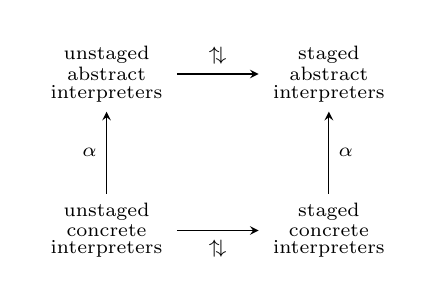
\begin{tikzpicture}
  \matrix (m) [matrix of math nodes,row sep=3em,column sep=3em,minimum width=2em]
  {
    \begin{smallmatrix} \text{unstaged} \\ \text{abstract} \\ \text{interpreters} \end{smallmatrix} & \begin{smallmatrix} \text{staged} \\ \text{abstract} \\ \text{interpreters} \end{smallmatrix} \\
      \begin{smallmatrix} \text{unstaged} \\ \text{concrete} \\ \text{interpreters} \end{smallmatrix} & \begin{smallmatrix} \text{staged} \\ \text{concrete} \\ \text{interpreters} \end{smallmatrix} \\ };
  \path[-stealth]
    (m-1-1) edge node [above, font=\scriptsize] {$\updownarrows$} (m-1-2)
    (m-2-1) edge node [left, font=\scriptsize] {$\alpha$} (m-1-1)
    (m-2-1) edge node [below, font=\scriptsize] {$\updownarrows$} (m-2-2)
    (m-2-2) edge node [right, font=\scriptsize] {$\alpha$} (m-1-2);
  \end{tikzpicture}
  \caption{The confluence of specialization and approximation.}
  \label{confluence}
\end{figure}

In this paper, we study the confluence of two old ideas --- Futamura projection
and abstract interpretation, but from the perspective of their recent
realizations --- multi-stage programming and definitional abstract interpreters.
To be specific, we present the application of the first Futamura projection on
definitional abstract interpreters, which intersects as staged abstract
interpreters. By borrowing the ideas from monadic interpreters
\cite{Steele:1994:BIC:174675.178068, DBLP:conf/popl/LiangHJ95,
DBLP:journals/pacmpl/DaraisLNH17, Sergey:2013:MAI:2491956.2491979} and embedded
domain-specific languages \cite{DBLP:conf/snapl/RompfBLSJAOSKDK15,
DBLP:journals/jfp/CaretteKS09, DBLP:conf/icfp/GibbonsW14,
Hofer:2008:PED:1449913.1449935}, we develop an approach to fulfill four
different semantics (Figure~\ref{confluence}) in a unified framework. The four
semantics share one same generic interpreter interface. Later, by instantiating
the interpreter differently, it can behave as a concrete interpreter, an
abstracter interpreter, or their code-generator versions, respectively. The key
idea that enables this flexibility is to use abstract type members abstract over
concrete/abstract components (e.g., concrete values or abstract values), as well
as the binding-time of them (e.g., static or dynamic). By staging, the overhead
caused by the monadic layers is eliminated in the generated code.

\paragraph{Performance via Specialization}

Besides the intellectual merit shown in the confluence diagram, this paper
contributes to a practical problem in static analysis: \textit{can we speed up a
static analyzer without any intrusive changes and soundness compromises?} Static
analysis is known as a trade-off game between \textit{precision} and
\textit{efficiency}, we argue that applying meta-programming (multi-stage
programming, in particular) with abstract interpreters is an effective approach
to improve the latter one while the former one is untouched. Specialization
removes the overhead of abstractions introduced by high-level programming (e.g.,
monads), but not loses any advantages of this programming style (e.g.,
extensibility), nor changes the meaning of the program -- in this case, the
abstract semantics that does the analysis. Indeed, specializing analysis
with respect to a program by partial evaluation \cite{damian1999partial,
amtoft1999partial, Boucher:1996:ACN:647473.727587, ashley:practical} is not a
new idea, despite the fact that most of the previous work are ad-hoc on a
particular analysis or requiring significant changes to the analysis. For
example, abstract compilation \cite{Boucher:1996:ACN:647473.727587} requires the
whole analyzer to be rewritten as closure generation from. In this paper, we
show a systematic approach to meta-programming that achieves the performance
goal with less intrusive changes; in fact, a case study (Section~\ref{cs_ac})
comparing with abstract compilation shows, by utilizing type-based stage
annotations, the analyzer program does not need any changes.

\paragraph{Modularity via Meta-Programming}

Our second contribution is to enable modular analysis based on a whole-program
analyzer by meta-programming. Modern software are shipped with large libraries
\cite{toman_et_al:LIPIcs:2017:7121}, and analyzing programs with large libraries
is usually expensive or unnecessarily repeated for whole-program analyzing
algorithms. For example, it has been shown that analyzing a simple ``Hello
World'' program in Java depends on additional 3,000 classes in the library
\cite{DBLP:conf/oopsla/KulkarniMZN16}. A natural idea is to analyze libraries
and generate summaries, later we can plugin the necessary information into the
summaries and finish the analysis; therefore such summaries should be modular
and reusable. Meta-programming gives us a chance to readily tweak a
whole-program analyzing algorithm into an analyzer that works modularly and
produces summaries. Still, the idea is to specialize the abstract interpreter
that was used for whole-program analysis, but on a subset of the program, for
examples, several generic functions for list manipulation. Such specialization
works on lambda expressions and generates code, which is partial analysis
results and can be completed by running with the necessary arguments (for
example, an environment that closes the lambda term) at next stages. Multiple
partial analysis results also can be reused later and composed together as they
are just normal programs at the next stage. Through staging, we mechanically
obtain a modular analysis, even though the original algorithm is formulated as a
whole-program analysis.

\iffalse
Likewise, specializing static analyses by partial evaluation emerged in late 90s
, and indeed it is able to effectively remove the interpretive
overhead of repeatedly traversing the abstract syntax tree. However, these
previous works focused mostly on one particular analysis, or required to
completely rewrite the analyzer. Hence, it is worth to investigate the idea from
a modern perspective based on generative programming, especially for a general
abstract interpreter that models direct-style $\lambda$-calculus, imperative
features such as mutation, and different abstract domains. One technical
challenge is the binding-time engineering when non-determinism, fixed-point
iterations, different abstract domains and staging are introduced at the same
time. In this paper, we present an end-to-end design and implementation of
staging an abstract interpreter; that means not only the interpreter that
traverses the abstract syntax tree, but also the data structure of abstract
domains, abstract environment and heap, and the fixed-point iteration are
staged.

\todo{rewrite this paragraph}
On the other hand, the abstract interpreter, as a semantic artifact, should be
written in a style that is easy for people to communicate the formulation and
abstraction, but also can be implemented efficiently. As the slogan of
multi-stage programming said, "abstraction without regret", we draw connection
between high-level description and efficient implementation of abstract
interpreters, just like the connection between concrete interpreters and
compilers drawn by Futamura projection. Particularly, we show an easy but
systematic way of adding stage annotations to the abstract interpreter without
changing the code of the interpreter skeleton, which is shared between four concrete
or abstract, unstaged or staged interpreters. We use the LMS framework for staging,
which allows us only use types to annotate the binding-time. Therefore, the
proposed approach bridges the gap between designing sound static analysis and
implementing efficient program analyzer.

%Of course, all interpreters are metalinguistic abstractions, but some
%interpreters are more "abstract" than others \todo{maybe rephrase}.
%Particularly, we also would like a systematic approach to optimize program
%analyzers and meanwhile minimally modifying the analyzer programs.

When staging a concrete interpreter, the programmers need to distinguish static
and dynamic values --- the given program to be executed by the interpreter is
classified as static because it is known at compile-time, and the inputs to that
program are dynamic. However, when staging an abstract interpreter, this
distinction does not exist anymore. Because the abstract interpreter
instantiates all the inputs as some form of abstract values, which are usually
top elements in their abstract domains and are also statically known. Then what
is the point of staging if there is no such distinction? A surprising by-product
of thinking about this question is to realize that we can apply the staged
abstract interpreter on \textit{open} programs, and the free variables
representing other parts of the program (e.g., libraries) are dynamic inputs,
therefore we obtain a modular analysis through staging, mechanically.
\note{TR: I don't understand this. The program structure is static, the abstract values
are still dynamic, no? They change in every iteration of the fixpoint algorithm}
\note{TR: why is it a big deal. On Closed programs we obtain a constant factor,
but modular analysis has different asymptotics}

When targeting higher-order programs, either staged concrete interpreters or
staged abstract interpreters are able to compile a closure, i.e., specialize the
call of interpreter with respect to the body expression of the lambda term
without knowing the actual argument value. By generalizing this observation, we
can actually specialize the abstract interpreter with any open programs, which
unexpectedly leads to a modular analysis and improves scalability. An open
program contains free variables, which represent other parts of the program and
will be left as dynamic values. For instance, one challenge in static analysis
of modern software is that the programs are usually shipped with large library
code \cite{toman_et_al:LIPIcs:2017:7121}, for example, it has been shown that
analyzing a simple "Hello World" program in Java depends on additional 3,000
classes in the library \cite{DBLP:conf/oopsla/KulkarniMZN16}. A precise
whole-program analysis formulated as abstract interpreters can be very expensive
due to the scale of the program and the inherent complexity of the algorithm.
However, analyzing these libraries is sometimes unnecessarily repeated. When
applying the staged abstract interpreter on such open programs, we leave the
unknown arguments and calling contexts as dynamic values and generate partial
analyzing result which is represented as a residual program. The partial
analyzing result can be reused and composed with the analyzing result of
application code when available later. Therefore we mechanically obtain a
modular analysis through staging, even though the original algorithm is
formulated as a whole-program analysis.

It has been observed that partially applying context-sensitivity on selected
portion of the program could improve the precision and efficiency
\cite{zipper2018, Kastrinis:2013:HCP:2491956.2462191}. We show that staging
abstract interpreters as an approach to effectively implement hybird
context-sensitivity\todo{}.
\fi

%\note{Expression problem \cite{DBLP:conf/icfp/GibbonsW14, DBLP:conf/ecoop/KrishnamurthiFF98, expproblem},}

\paragraph{Contributions and Outline}

\begin{itemize}
  \item We progressively present a unifying construction that naturally extends
    the first Futamura projection to abstract interpreters. Starting from a generic
    interface of the interpreter for a small functional language
    (Section~\ref{generic_if}), we first show the instantiation of concrete
    interpretation (Section~\ref{unstaged_conc}). Then we lift it to the staged
    version by replacing the binding-time type (Section~\ref{stagedinterp}); and to
    the abstract interpreter by applying abstraction to the environment, store, and
    values (Section~\ref{unstaged_abs}). Finally, we show the combination of the two
    transformations, dubbed \textit{staged abstract interpreters}, can be easily
    derived (Section~\ref{sai}).

  \item We demonstrate that if we apply the abstract interpreter on components
    of the program separately, it not only improves the \textit{efficiency} but
    also the \textit{scalability} (Section~\ref{sai} \todo{}), which are two
    major issues in static analysis.

  \item We conduct two case studies to show the applicability and usefulness
    of applying meta-programming to static analysis (Section~\ref{cases_study}).
    (1) We first revisit the Abstract Compilation (AC)
    \cite{Boucher:1996:ACN:647473.727587} technique (Section~\ref{cs_ac}).
    Our approach and AC are able to achieve the same goal, however, as we show,
    one of the advantage of staging through types is it does not require
    whole-analyzer refactoring.
    (2) We extend the staged abstract interpreter to two variants of
    control-flow analysis: context-sensitive pushdown control-flow analysis and
    \todo{precise-store?} (Section~\ref{sai}).
    
  \item Based on the instantiation of control-flow analysis, we empirically
    evaluate the performance improvement by staging and specialization
    (Section~\ref{evaluation}). We compare the both context-insensitive and
    \note{context-sensitive} analysis.
    
\end{itemize}

\newcommand{\TLang}{$L_\lambda$}

\section{Preliminaries} \label{prelim}

In this section, we first describe the abstract syntax of the language. Then,
we present the generic interpreter shared among the four different semantics,
after which we instantiate the interpreter to the concrete one. It is worth
noting that we choose to use Scala and a monadic style to demonstrate this
idea, though the approach is not restricted to this choice.  Indeed, one can
use imperative or direct-style in other MSP languages (e.g., MetaOCaml
\cite{DBLP:conf/gpce/CalcagnoTHL03, DBLP:conf/flops/Kiselyov14} or Template
Haskell \cite{Sheard:2002:TMH:636517.636528}) to construct such staged abstract
interpreters, although the details are different.

\subsection{Abstract Syntax} \label{bg_lang}

We consider a call-by-value $\lambda$-calculus in direct-style, extended with
numbers, arithmetic, recursion, and conditionals. Other effects such as
assignments can also be supported readily. Since we are interested in
analyzing the dynamic behavior of programs, we elide the static semantics. We also
assume that input programs are well-typed and all variables are distinct. The
abstract syntax is as follows:
\begin{lstlisting}
  abstract class Expr
  case class Lit(i: Int) extends Expr                         // numbers
  case class Var(x: String) extends Expr                      // variables
  case class Lam(x: String, e: Expr) extends Expr             // abstractions
  case class App(e1: Expr, e2: Expr) extends Expr             // applications
  case class If0(e1: Expr, e2: Expr, e3: Expr) extends Expr   // conditionals
  case class Rec(x: String, rhs: Expr, e: Expr) extends Expr  // recursion
  case class Aop(op: String, e1: Expr, e2: Expr) extends Expr // arithmetic
\end{lstlisting}

The abstract syntax we present can be seen as a deep embedding of the language:
we use data-types to represent programs. This is the most natural choice
for program analysis and allows us to use different interpretations over the
AST; with the inheritance and overriding mechanisms in Scala, we may also add
new language constructs and reuse existing interpretations.

%\todo{cite Bruno?}.

\iffalse
We will give the concrete semantics using a big-step definitional
interpreter. The interpreter is a recursive function that takes the program AST,
environment, and store, and returns the evaluated value and the accompanying
store. The environment is a mapping from identifiers to addresses, and the store
is a mapping from addresses to values. We use the store to model recursion and
mutation in concrete semantics; it is also useful for polyvariant analysis. This
environment-and-store-passing style big-step interpreter is standard and can
also be obtained by refunctionalizing \cite{DBLP:conf/ppdp/AgerBDM03,
Wei:2018:RAA:3243631.3236800} a small-step CESK machine
\cite{DBLP:conf/popl/FelleisenF87}.
\fi

\subsection{Monads in Scala} \label{monadscala}

A monad is a type constructor @M[_]: * --> *@ with two operations, often called
@return@ and @bind@ \cite{Wadler:1992:EFP:143165.143169,
DBLP:journals/iandc/Moggi91}. Informally, @return@ wraps a value into a monad
@M@, and @bind@ unwraps a monadic value and transforms it into a new monadic value.
Pragmatically in Scala, we define the monad type class using trait @Monad@
(Figure \ref{fig:monad}), which declares the @pure@ \footnote{We elect to use
\texttt{pure} as the name, since \texttt{return} is a keyword in Scala and
\texttt{unit} is a built-in function in LMS.} and @flatMap@ operations. The
trait itself takes the monad type constructor @M[_]@ as an argument, which, as a
higher-kinded type, takes a type and returns a type. The method @pure@ promotes
values of type @A@ to values of type @M[A]@. The monadic @bind@ operation is
usually called @flatMap@ in Scala. It takes a monad-encapsulated value of type
@M[A]@, a function of @A => M[B]@, and returns values of type @M[B]@.

\begin{figure}[h!]
  \centering
  \vspace{-1em}
  \begin{subfigure}[b]{0.55\textwidth}
    \begin{lstlisting}
  trait Monad[M[_]] {
    def pure[A](a: A): M[A]
    def flatMap[A,B](ma: M[A])(f: A => M[B]): M[B]
  }
    \end{lstlisting}
    \vspace{-0.5em}
    \caption{trait \texttt{Monad}} \label{fig:monad}
  \end{subfigure}
  ~
  \begin{subfigure}[b]{0.4\textwidth}
    \begin{lstlisting}
trait MonadOps[M[_], A] {
  def map[B](f: A => B): M[B]
  def flatMap[B](f: A => M[B]): M[B]
}
    \end{lstlisting}
    \vspace{-0.5em}
    \caption{trait \texttt{MonadOps}} \label{fig:monadops}
  \end{subfigure}
\end{figure}
\vspace{-1em}

Similar to Haskell's @do@-notation, Scala provides special syntactic support
for monadic operations through @for@-comprehension.  For example, an object of
@List[A]@ is an instance of the @List@ monad, with element type @A@.
To compute the Cartesian product of two lists of numbers, we can use Scala's
@for@-comprehension syntax:
\begin{lstlisting}
  val xs = List(1, 2); val ys = List(3, 4)
  for { x <- xs; y <- ys } yield (x, y)   // List((1,3), (1,4), (2,3), (2,4))
\end{lstlisting}

The Scala compiler translates the above @for@-comprehension expression into
an equivalent one using @flatMap@ and @map@. The last binding
in @for@-comprehensions is translated into a @map@ operation, where the argument of
@yield@ becomes the body expression inside that @map@ operation. The
bindings before the last one are all translated into calls of @flatMap@:
\begin{lstlisting}
  xs.flatMap { case x => ys.map { case y => (x, y) } }
\end{lstlisting}

Note that here the monadic object @List[_]@ encapsulates the data internally.
Therefore, it only exposes the simplified version of @flatMap@, where the monadic
value of @M[A]@ is not introduced as a function argument. The trait @MonadOps@ (Figure
\ref{fig:monadops}) defines the simplified versions of monadic operations that
are necessary for @for@-comprehension. The conversion between @Monad@ and
@MonadOps@ can be achieved by using the implicit design pattern.
In the rest of the paper, we use Scala's @for@-comprehension syntax and a few
monads and monad transformers such as @ReaderT@, @StateT@, and @SetT@ to
write our interpreters.
Monad transformers are type constructors of kind @(* --> *) --> (* --> *)@, which
take a monad as an argument and produce another monad. By using monad
transformers, we can combine multiple monads into a single one.  The
implementation of monads and monad transformers follows the ones from Haskell.

\subsection{Generic Interpreter} \label{generic_if}

In this section, we present the generic evaluator interface in the style of a big-step
definitional interpreter. The key idea is to keep both the binding-time type and
returned monadic type abstract, so that they can be instantiated
differently. We also need to abstract the primitive operations on those types.
In later sections, we will instantiate the monadic type to perform concrete
interpretation \cite{DBLP:conf/popl/LiangHJ95} or abstract interpretation
\cite{Sergey:2013:MAI:2491956.2491979, DBLP:journals/pacmpl/DaraisLNH17}.

\paragraph{Basic Types} We start with some basic type definitions that are used
in the interpreter. The identifiers in the program are represented by strings.
To represent states, two required components for the interpreter are
environments, represented by type @Env@, and stores, represented by type
@Store@. An @Env@ maps identifiers to addresses, and a @Store@ maps addresses to
values. An environment captures bound variables in the scope of current control, and
a store models a persistent heap through the program run-time.  Currently,
the domains of addresses and values are still abstract; hence, they are
declared as abstract types.
\begin{lstlisting}
  trait Semantics {
    type Ident = String; type Addr; type Value
    type Env = Map[Ident, Addr]; type Store = Map[Addr, Value]
    type R[_] // Binding-time as a higher-kinded type
    ... // The definitions in the rest of this section are enclosed in trait Semantics.
  }
\end{lstlisting}

\paragraph{Binding-time Abstraction}
The binding-time type is declared as a higher-kinded type @R[_]@ \cite{Ofenbeck:2017:SGP:3136040.3136060}.
Now we can use @R@ to annotate other data-types in the interpreter;
it is also injected into the monadic type @MonadOps@.  If we instantiate
@R@ as the identity type (i.e., @type R[T] = T@), then the generic interpreter is a
standard definitional interpreter that will execute the program.  In Section
\ref{stagedinterp}, we instantiate @R@ using LMS's built-in next-stage
type annotation @Rep@, which makes the interpreter act as a compiler.

\paragraph{Monadic Operations} We define the return type of the interpreter
@Ans@ as a monadic type @AnsM[_]@ wrapping the type @Value@.
As mentioned in Section~\ref{monadscala}, in order to use the @for@-comprehension
syntax certain operations must be added on the type @AnsM@. Here, we use a
structural type @MonadOps@ to require that type @AnsM@ must (at least)
implement @map@ and @flatMap@. It is worth noting that @MonadOps@ takes another
type parameter @R[_]@ as the binding-time, i.e., @MonadOps[R, AnsM, T]@.
Inside @MonadOps@, @R[_]@ annotates the data types @A@ and @B@ that are
encapsulated by the monad, but not the monad type @M@ itself. When the generic
interpreter acts as a compiler, we will replace the monads with the ones that
work on staged data values.

We also declare several operations to manipulate environments and
stores. These methods return monadic values of type @AnsM[_]@, which
may be parameterized over the environment or store type, or merely a @Unit@
value for performing effects. For example, @local_env@ installs a new environment
@ρ@ when evaluating the monadic value @ans@; @set_store@ takes a pair of
addresses and (potentially staged) values, and updates the store accordingly.

%\vspace{-1em}
\begin{figure}[h!]
  \centering
\vspace{-1em}
  \begin{subfigure}[b]{0.45\textwidth}
    \begin{lstlisting}
  type MonadOps[R[_], M[_], A] = {
    def map[B](f: R[A] => R[B]): M[B]
    def flatMap[B](f: R[A] => M[B]): M[B]
  }

  type AnsM[T] <: MonadOps[R, AnsM, T]
  type Ans = AnsM[Value]
    \end{lstlisting}
  \end{subfigure}
  ~
  \begin{subfigure}[b]{0.55\textwidth}
    \begin{lstlisting}
// Environment operations
def ask_env: AnsM[Env]
def local_env(ans: Ans)(ρ: R[Env]): Ans
// Store operations
def get_store: AnsM[Store]
def put_store(σ: R[Store]): AnsM[Unit]
def set_store(av: (R[Addr], R[Value])): AnsM[Unit]
    \end{lstlisting}
  \end{subfigure}
\end{figure}
\vspace{-1em}

\paragraph{Primitive Operations} Next, we define a few primitive operations.
First, we declare two versions of @alloc@. The first takes a store and an
identifier and produces a fresh address of non-monadic type @R[Addr]@. Since
the freshness of the address may depend on the store, which might be a
next-stage value as indicated by its type, the type of addresses is
consequently wrapped by @R[_]@. The other @alloc@ is simply the monadic version
of the addresses, and can therefore be used in monadic computations.
An auxiliary method @get@ retrieves the value of an identifier @x@ through the
environment and store.
\begin{lstlisting}
  def alloc(σ: R[Store], x: Ident): R[Addr];  def alloc(x: Ident): AnsM[Addr]
  def get(σ: R[Store], ρ: R[Env], x: Ident): R[Value]
\end{lstlisting}

Other primitive operations in the interpreter handle the language constructs.  The
methods @num@ and @close@ deal with primitive values, which lift literal terms
(e.g., lambdas) to our value representation (e.g., closures).
Conditionals and arithmetic are handled by @br0@ and @arith@, respectively. The
method @ap_clo@ is used for applying functions, by taking a function value
and an argument value. Note that the @Env@, @Store@, and @Value@ are all
annotated by @R[_]@, as they are potentially next-stage values when the
interpreter acts as a compiler.
\begin{lstlisting}
  def num(i: Int): Ans
  def close(ev: Expr => Ans)(λ: Lam, ρ: R[Env]): R[Value]
  def br0(test: R[Value], thn: => Ans, els: => Ans): Ans
  def arith(op: Symbol, v1: R[Value], v2: R[Value]): R[Value]
  def ap_clo(ev: Expr => Ans)(fun: R[Value], arg: R[Value]): Ans
\end{lstlisting}

\begin{figure}[t]
  \centering
  \begin{lstlisting}
          def eval(ev: Expr => Ans)(e: Expr): Ans = e match {
            case Lit(i) => num(i)                   case Let(x, rhs, e) => for {
            case Var(x) => for {                      v  <- ev(rhs)
              ρ <- ask_env                            ρ  <- ask_env
              σ <- get_store                          α  <- alloc(x)
            } yield get(σ, ρ, x)                      _  <- set_store(α → v)
            case Lam(x, e) => for {                   rt <- local_env(ev(e))(ρ + (x → α))
              ρ <- ask_env                          } yield rt
            } yield close(ev)(Lam(x, e), ρ)         case Aop(op, e1, e2) => for {
            case App(e1, e2) => for {                 v1 <- ev(e1)
              v1 <- ev(e1)                            v2 <- ev(e2)
              v2 <- ev(e2)                          } yield arith(op, v1, v2)
              rt <- ap_clo(ev)(v1, v2)              case Rec(x, rhs, e) => for {
            } yield rt                                α  <- alloc(x)
            case If0(e1, e2, e3) => for {             ρ  <- ask_env
              cnd <- ev(e1)                           v  <- local_env(ev(rhs))(ρ + (x → α))
              rt  <- br0(cnd, ev(e2), ev(e3))         _  <- set_store(α → v)
            } yield rt                                rt <- local_env(ev(e))(ρ + (x → α))
                                                    } yield rt
          }
  \end{lstlisting}
\vspace{-0.5em}
\caption{The generic interpreter,
  shared by the unstaged/staged + concrete/abstract interpreter.}
\vspace{-1.5em}
\label{fig:shared_int}
\end{figure}

\paragraph{The Interpreter} We can now construct the semantics-agnostic interpreter
in monadic form, as shown in Figure \ref{fig:shared_int}. The basic idea
of generic interpretation is to traverse the AST
while maintaining the effects (such as environment and state updates).
Note that the interpreter is written in open-recursive style: it cannot
refer to itself directly. Instead, @eval@ takes an additional parameter @ev@ of
type @Expr => Ans@ that refers to itself. Consequently, method @close@ that
lifts $\lambda$-terms to closures and method @ap_clo@ that applies functions also
takes an extra @ev@, because further evaluation may happen inside them.
To close the open recursion, we use a fixed-point operator @fix@.
For concrete-interpretation instantiation, @fix@ works like the Y combinator;
for abstract-interpretation instantiation, it will instrument the interpreter
by memoizing @ev@'s inputs and outputs, which ensures the termination of
abstract interpretation.
Finally, there is a top-level wrapper @run@. The return type @Result@
depends on the kind of monads being used and is therefore also left abstract.
\begin{lstlisting}
  def fix(ev: (Expr => Ans) => (Expr => Ans)): Expr => Ans
  type Result; def run(e: Expr): Result
\end{lstlisting}

%==========================================================================

\section{A Concrete Interpreter} \label{unstaged_conc}

As the first step in our roadmap, we instantiate the generic interpreter for
concrete execution in this section. The result is a standard definitional
interpreter with environments and stores. It can also be obtained by
refunctionalizing a standard CESK machine \cite{Felleisen:1987:CAH:41625.41654,
DBLP:conf/ppdp/AgerBDM03}. We first present the concrete components, i.e., the
value domains, then show the monad stack for concrete interpretation, and finally
sketch how the primitive operations are implemented.

\paragraph{Concrete Components}
The two types we need to concretize are addresses @Addr@ and values @Value@. The
types @Env@ and @Store@ are derived automatically. To ensure the freshness of
address allocations, we use type @Int@ and always return a number that is greater
than the size of the current store.
A value can be either a tagged number \texttt{IntV}, or a closure
\texttt{CloV} that contains a $\lambda$-term and an environment. The final
result of the interpreter is a pair of values and stores.
To distinguish from the monadic values of type @Ans@ produced by the
interpreter, later we use term \textit{grounded values} to denote such final values.
The two elements in the type @Result@ are annotated by the binding-time @R@,
because they can be next-stage objects.  We also define a standard fixed-point
combinator to close the open-recursive function @ev@.
\begin{lstlisting}
  trait ConcreteComponents extends Semantics {
    type Addr = Int;  sealed trait Value
    case class IntV(i: Int) extends Value
    case class CloV(λ: Lam, e: Env) extends Value
    type Result = (R[Value], R[Store])
    def fix(ev: (Expr => Ans) => (Expr => Ans)): Expr => Ans = e => ev(fix(ev))(e)
  }
\end{lstlisting}

\paragraph{Unstaged Monads}
For concrete interpretation, the monad needs to model reader and state effects,
which correspond to the environment and the store, respectively. We follow the
monad transformer approach \cite{DBLP:conf/popl/LiangHJ95},
and use the @ReaderT@ and @StateT@ monad transformers to
compose the monad stack. In other words, the type @AnsM@ is
instantiated by layering the @ReaderT@ and @StateT@ transformers\footnote{The
question mark syntax is a kind projector \cite{kindprojector}, such that
\texttt{StateT[IdM,Store,?]} is equivalent to \newline \texttt{(\{type
M[T]=StateT[IdM,Store,T]\})\#M}}, where the @ReaderT@ is parameterized by the
type @Env@, and the @StateT@ is parameterized by the type @Store@, and the
inner-most monad @IdM@ is merely the identity monad.
\begin{lstlisting}
  trait ConcreteSemantics extends ConcreteComponents {
    type R[T] = T
    type AnsM[T] = ReaderT[StateT[IdM, Store, ?], Env, T] // the monad stack
    ... }
\end{lstlisting}

Here, we sketch the basic idea of @ReaderT@ and @StateT@. Readers may
refer to \cite{DBLP:conf/popl/LiangHJ95, Chiusano:2014:FPS:2688794} for more detail.
A @ReaderT@ monad transformer encapsulates computation @R => M[A]@, where
@R@ is the environment type, and @M[_]@ is the inner monadic type.
Given a value of @R@, a @ReaderT@ monad produces a transformed value of type @M[A]@.
Similarly, a @StateT@ monad encapsulates computation @S => M[(A, S)]@, where
@S@ is the state type, and @M[_]@ is the inner monad type.
Given a value of type @S@, a @StateT@ monad produces a transformed value of type @M[(A, S)]@,
where the new state (of type @S@) is accompanied with the result (of type @A@).
Note that for the moment, the binding-time type @R@ is the identity type; thus,
these monads operate on unstaged data. We can also see this from the
signature of @flatMap@: the argument function @f@ takes an unstaged value of type @A@ and
produces a monadic value. In the following code, we elide operations other than @flatMap@.
\begin{lstlisting}
  case class ReaderT[M[_]: Monad, R, A](run: R => M[A]) {
    def flatMap[B](f: A => ReaderT[M, R, B]): ReaderT[M, R, B] =
      ReaderT(r => Monad[M].flatMap(run(r))(a => f(a).run(r))); ... }
  case class StateT[M[_]: Monad, S, A](run: S => M[(A, S)]) {
    def flatMap[B](f: A => StateT[M, S, B]): StateT[M, S, B] =
      StateT(s => Monad[M].flatMap(run(s)) { case (a, s1) => f(a).run(s1) }); ... }
\end{lstlisting}

After defining the monad stack, the operations manipulating environments
and stores can be defined by constructing the proper monadic value and lifting it to the
top-level of our monad stack. To modify the store, for example, we construct a
@StateT@ value that updates the current store $\sigma$ to @σ + αv@, which
results in a @StateT[IdM, Store, Unit]@ value. Then, we lift this @StateT@
value to the top-level @ReaderT@ type, i.e., @AnsM[Unit]@.
\begin{lstlisting}
  def set_store(αv: (Addr, Value)): AnsM[Unit] = liftM(StateTMonad.mod(σ => σ + αv))
\end{lstlisting}

\paragraph{Primitive Operations}
Other primitive operations over the value domains can be implemented
straightforwardly. We elide most of them but describe how we handle
functions and applications. The reason is that $\lambda$-terms are data but are also
part of the control flow. The way we treat them is simple now, but
will become more involved when we stage the abstract interpreter.
The method @close@ denotes a $\lambda$-term to our representation of functions.
At the moment, @close@ takes a $\lambda$-term and an environment, and
produces the defunctionalized representation of closures.
The method @ap_clo@ performs function applications, which takes a function
value @fun@ and an argument @arg@. It first extracts the syntactic
$\lambda$-term and environment enclosed in @fun@, and allocates an addresses
for the argument and updates the environment and store accordingly.  Finally,
by recursively calling @ev@, it evaluates the body expression of the
$\lambda$-term under the new environment and store.
\begin{lstlisting}
  def close(ev: Expr => Ans)(λ: Lam, ρ: Env): Value = CloV(λ, ρ)
  def ap_clo(ev: Expr => Ans)(fun: Value, arg: Value): Ans = fun match {
    case CloV(Lam(x, e), ρ: Env) => for {
      α <- alloc(x)
      _ <- set_store(α → arg)
      rt <- local_env(ev(e))(ρ + (x → α))
    } yield rt
  }
\end{lstlisting}

We define the top-level @run@ method as invoking the fixed-point operator with
the evaluator and input expression @e@, and running the monad stack with the
initial environment $\rho_0$ and store $\sigma_0$.
\begin{lstlisting}
  def run(e: Expr): Result = fix(eval)(e)(ρ$_0$)(σ$_0$)
\end{lstlisting}

\section{From Interpreters to Staged Interpreters} \label{stagedinterp}

In this section, based on the generic interpreter and concrete components we
presented in Section \ref{prelim}, we show how to stage the concrete
interpreter by changing the monad type and refactoring the primitive
operations. We begin by briefly introducing the Lightweight Modular Staging
framework in Scala, and then replay the same steps as we did for the unstaged
counterpart. Finally, we briefly describe the code generation.

\subsection{Multi-stage Programming with LMS}

Lightweight Modular Staging (LMS) \cite{DBLP:conf/gpce/RompfO10} is a
multi-stage programming framework implemented as a Scala library. LMS enables
runtime code generation in a type-safe manner. Different from the approach of
MetaML/MetaOCaml \cite{DBLP:conf/flops/Kiselyov14, DBLP:conf/gpce/CalcagnoTHL03} which
uses syntactic quotations, LMS distinguishes binding-times based on types. 
To achieve this, LMS provides a type constructor @Rep[T]@, where @T@ can be an
arbitrary type, indicating that a value of type @T@ will be known at a future
stage.  Operations acting on @Rep[T]@ expressions will be residualized as
generated code.
A classic example for introducing multi-stage programming is the power function
that computes $b^x$. Usually, it is implemented as a recursive function:
\begin{lstlisting}
  def power(b: Int, x: Int): Int = if (x == 0) 1 else b * power(b, x - 1)
\end{lstlisting}

If @x@ is known at the current stage, we may specialize the power function to
the value @x@ by unrolling the recursive calls. In LMS, this is fulfilled by
first adding the @Rep@ type annotation to variables known at the next stage. In this case,
@b: Rep[Int]@ is known later, and @x: Int@ is known currently, as shown below.
The way we use this staged @power@ function is to create a @DslDriver@ and override the
@snippet@ method that supplies 5 as the currently known value for @x@.
\begin{lstlisting}
  new DslDriver[Int, Int] {
    def power(b: Rep[Int], x: Int): Rep[Int] = if (x == 0) 1 else b * power(b, x-1)
    def snippet(b: Rep[Int]): Rep[Int] = power(b, 5) // specialize the power to b^5
  }
\end{lstlisting}

The LMS framework provides staging support for primitive data types such as
@Int@ and @Double@, and for commonly-used data structures such as lists and
maps.  The framework internally constructs a sea-of-nodes intermediate
representation (IR) for the next-stage program when executing the current stage
program \cite{DBLP:conf/birthday/Rompf16}.
For convenience, the conversion from expressions of type @Rep[_]@ to their IR
is done by using the implicit design pattern. As we will see later,
implementing staging and code generation support for user-defined classes is
also straightforward.

\subsection{Staged Concrete Semantics}

To implement the staged concrete interpreter, we replay the steps from the
instantiation of the unstaged counterpart in Section \ref{unstaged_conc}.
However, now we use the @Rep@ type to annotate the value domains, environments and
stores, and define the staged version of monads and primitive operations.

\paragraph{Staged Monads}
We use the same monad stack structure as in the unstaged interpreter: a reader
monad with a state monad. The difference here is that, now the monads operate
on staged values.  For brevity, we call them \textit{staged monads}. In the
code snippet, we also use a @Rep@ prefix on the name of constructors and types
to differentiate them.
But it is important to note that the instances of @ReaderT@/@StateT@ are not
staged, and that the monadic computation, such as functions of @R => M[A]@, are
also not staged. Instead, the internal data that these monads operate on are
staged, i.e., values of type @R@ and @A@ in the reader monad, and values of type @S@ and
@A@ in the state monad.
The following code snippet shows the idea. We use \hl{light gray} to highlight
where @Rep@ types are added.
\begin{lstlisting}[escapechar=!]
  case class RepReaderT[M[_]: RepMonad, R, A](run: !\hl{Rep[R]}! => M[A]) {
    def flatMap[B](f: !\hl{Rep[A]}! => ReaderT[M, R, B]): RepReaderT[M, R, B] =
      RepReaderT(r => RepMonad[M].flatMap(run(r))(a => f(a).run(r))); ... }
  case class RepStateT[M[_]: RepMonad, S, A](run: !\hl{Rep[S]}! => M[(A, S)]) {
    def flatMap[B](f: !\hl{Rep[A]}! => StateT[M, S, B]): RepStateT[M, S, B] =
      RepStateT(s => RepMonad[M].flatMap(run(s))(as => f(as._1).run(as._2))); ... }
\end{lstlisting}

The function @f@ passed to the @flatMap@ is also a value known at the current stage.
Therefore, all invocations of @flatMap@ can be reduced before generating code.
The fact that we only stage data but not the monadic computation or monadic
values is the reason that we can peel of the monad stack in the generated code
through staging.  Now the type @AnsM[_]@ is instantiated as the same structure
as before, but using the @Rep@ versions of monad transformers:
\begin{lstlisting}
  type R[T] = Rep[T]
  type AnsM[T] = RepReaderT[RepStateT[RepIdM, Store, ?], Env, T]
\end{lstlisting}

Readers may notice that the conversion between unstaged monads and staged monads
is merely changing the type of unstaged data to staged data, which in fact can
be achieved without modifying the implementation of monads. This is true so far,
but as we will see, it is not as straightforward for the nondeterminism monad
(@SetT@) in the abstract interpreter, because not only the elements in the set are
staged, but the whole set is also staged, and we have no knowledge about how
many elements in the set. Therefore, any traversals over the set has to be
staged.  In this section, we explicitly distinguish the two versions of monadic
interfaces. Later, we will instantiate the staged set monad by manually fusing
the fragment of the monad stack inside @SetT@.

\paragraph{Primitive Operations} Most of the primitive operations can be easily
translated to their staged versions -- we just need to change the types.  As we
mentioned before, we will illustrate in detail how functions and applications
are handled.  One problem here is what should we do for $\lambda$ terms when
staging them? We cannot directly create a next-stage defunctionalized closure
for it, because that means we still need to interpret over these closures at the
next stage and the interpretation overhead has not been eliminated. 
The solution is to compile the $\lambda$ term with its environment by calling
the evaluator at the current stage. The result is generating a next-stage
Scala function. The evaluator is passed as @ev@ to the method @close@.
The following code implements the idea:
\begin{lstlisting}
  type ValSt = (Value, Store)
  def emit_compiled_clo(f: (Rep[Value], Rep[Store]) => Rep[ValSt], λ: Lam, ρ: Exp[Env]): Rep[Value]
  def close(ev: Expr => Ans)(λ: Lam, ρ: Rep[Env]): Rep[Value] = {
    val Lam(x, e) = λ
    val f: (Rep[Value], Rep[Store]) => Rep[ValSt] = { case (v: Rep[Value], σ: Rep[Store]) =>
        val α = alloc(σ, x)
        ev(e)(ρ + (unit(x) → α))(σ + (α → v))
    }; emit_compiled_clo(f, λ, ρ)
  }
\end{lstlisting}

In @close@, we first create a function @f@ that takes a next-stage value and
store, and returns staged values and stores. The function @f@ is a
current-stage and we then use @emit_complied_clo@ to denote it to a next-stage
Scala function.
The method @emit_compiled_clo@ produces current-stage representations of
next-stage function values, i.e., of type @Rep[Value]@.
Inside function @f@, we can access the evaluator via @ev@.
However, @ev@ produces a monadic value of type @AnsM@, which can only exist at
the current stage. To connect current-stage monadic values and future-stage
grounded values, the evaluator @ev@ is supplied with not only the body
expression @e@ to be specialized, but also with the prepared environment and
store.  By doing so, we have \textit{collapsed} the monadic values of @AnsM@ to
grounded values within staging; therefore in the future stage, there is no
monads.
\begin{lstlisting}
  def emit_ap_clo(fun: Rep[Value], arg: Rep[Value], σ: Rep[Store]): Rep[ValSt]
  def ap_clo(ev: EvalFun)(fun: Rep[Value], arg: Rep[Value]): Ans = for {
    σ  <- get_store
    vs <- lift[ValSt](emit_ap_clo(fun, arg, σ))
    _  <- put_store(vs._2)
  } yield vs._1
\end{lstlisting}

For function applications @ap_clo@, we have two \textit{next-stage} values @fun@
and @arg@. But what we can do with these values of type @Rep@ is limited. 
In fact, @fun@ does not have an intensional application operation we can use
directly. We only know that it is a current-stage representation of functions produced by @close@,
whose next-stage form is a Scala function.
With this fact, we can generate a next-stage function application for it, also
in our target language Scala. The method @emit_ap_clo@ produces a current-stage
representation of a next-stage function application, with necessary arguments
such as the latest store @σ@. Meanwhile, we still want the method @ap_clo@
implemented in monadic style, so that it can be smoothly connected with other
parts of the interpreter.  To achieve this, we lift the result values and
stores from the future stage into our current-stage monad stack, with a binding
@vs@.  Finally, we use @put_store@ to update the store with @vs._2@ and return
the value result @vs._1@ into the current-stage monadic value.

Now, compared with the unstaged interpreter, we observe a key difference of where
we use the evaluation function @ev@.  In the unstaged interpreter, the
invocation of @ev@ happens in @ap_clo@, i.e., at the application time; while in
the staged interpreter, we eagerly apply @ev@ when denoting the lambda terms to
our next-stage value domains, i.e., at the value-representation time.

\subsection{A Little Bit of Code Generation}

In the previous section, we showed the types of @emit_compiled_clo@ and
@emit_ap_clo@ without concrete implementations. In this section, we briefly
discuss the IR nodes generated by them and sketch the code generation.
We define the IR nodes @IRCompiledClo@ and @IRApClo@ using @case class@
extending from @Def[T]@. @Def[T]@ is a built-in type in the LMS framework,
representing next-stage value definitions of type @T@.
\begin{lstlisting}
  case class IRCompiledClo(f: Rep[(ValSt) => ValSt], λ: Lam, ρ: Rep[Env]) extends Def[Value]
  case class IRApClo(fun: Rep[Value], arg: Rep[Value], σ: Rep[Store]) extends Def[ValSt]
\end{lstlisting}

The IR nodes are manipulated by the LMS passes and finally generated as
next-stage Scala programs. To generate code, LMS provides an @emitNode@ method for
programmers to control over what code is generated for each kind of nodes. Here,
we match @IRCompiledClo@ and @IRApClo@, and generate definitions via
@emitValDef@ for them.  For compiled closures, we pass the function @f@ with its
accompanying syntactic term and environment to the next-stage value
representation @CompiledClo@. For applications, we know that @fun@ is
an instance of @CompiledClo@ at the next stage, and it has a callable field
@f@. Hence, we generate a next-stage function application @f(arg, σ)@.  The
invocations of @quote@ are used to generate proper names for other
next-stage values.
\begin{lstlisting}
override def emitNode(sym: Sym[Any], rhs: Def[Any]) = rhs match {
  case IRCompiledClo(f, λ, ρ) => emitValDef(sym, s"CompiledClo($\textdollar${quote(f)}, $\textdollar${quote(λ)}, $\textdollar${quote(ρ)})")
  case IRApClo(fun, arg, σ) => emitValDef(sym, s"$\textdollar$fun.f($\textdollar${quote(arg)}, $\textdollar${quote(σ)})")
  ... }
\end{lstlisting}

\section{From Interpreters to Abstract Interpreters} \label{unstaged_abs}

After seeing both unstaged and staged concrete interpreters, now we turn our
focus on abstract interpreters under the same framework. We will first present a
lattice framework with binding-time abstraction, but for the purpose of clearly
illustrating the idea, we will just use simple abstract domains such as power set
lattice or point-wise map lattice. Then we show the abstract components, namely
abstract values, abstract environments and abstract stores.
The abstract interpreter we present in this section is similar to
\citet{DBLP:journals/pacmpl/DaraisLNH17}'s, it is also
context/path/flow-insensitive by our choice.  In Section \ref{cfa}, we will
instantiate a commonly-used context-sensitive analysis;
\citet{Darais:2015:GTM:2814270.2814308} shows how to achieve path- and
flow-sensitivity by varying the monads, which is also applicable to our unstaged
or staged abstract interpreter.

\subsection{Stage Polymorphic Lattices} \label{stagedpoly_lat}

A complete lattice over set $S$ is a tuple of $\langle S, \sqsubseteq, \top,
\bot, \sqcup, \sqcap \rangle$, where $\sqsubseteq : S \to S \to Bool$ is the
ordering relation, $\sqcup: S \to S \to S$ is the join (least upper bound)
operator, and $\sqcap: S \to S \to S$ is the meet (greatest lower bound)
operator. The trait @SPLattice@ (Figure \ref{fig:splattice}) defines the type
class of stage polymorphic lattices. Similar to @MonadOps@ in Section
\ref{generic_if}, we introduce an additional higher-kinded type @R[_]@ to
annotate the binding-times, where @R[_]@ wraps @S@ and @Boolean@ in these
operations.

\begin{figure}[h!]
  \centering
  \begin{subfigure}[b]{0.45\textwidth}
  \begin{lstlisting}[style=small]
trait SPLattice[S, R[_]] {
  val ⊤: R[S];  val ⊥: R[S]
  def ⊑(l1: R[S], l2: R[S]): R[Boolean]
  def ⊔(l1: R[S], l2: R[S]): R[S]
  def ⊓(l1: R[S], l2: R[S]): R[S]
}
trait Lattice[S] extends SPLattice[S, NoRep]
  \end{lstlisting}
  \caption{trait \texttt{SPLattice} and \texttt{Lattice}} \label{fig:splattice}
  \end{subfigure}
  ~
  \begin{subfigure}[b]{0.6\textwidth}
\begin{lstlisting}[style=small]
def SetLattice[T]: Lattice[Set[T]] = new Lattice[Set[T]] {
  lazy val ⊥: Set[T] = Set[T]()
  lazy val ⊤: Set[T] = error("No representation for ⊤")
  def ⊑(l1: Set[T], l2: Set[T]): Boolean = l1 subsetOf  l2
  def ⊔(l1: Set[T], l2: Set[T]): Set[T]  = l1 union     l2
  def ⊓(l1: Set[T], l2: Set[T]): Set[T]  = l1 intersect l2
}
\end{lstlisting}
  \caption{The power set instance for lattice} \label{fig:powerset}
\end{subfigure}
\end{figure}

In this section, we simply let @R[T] = T@ (i.e., @NoRep@) to instantiate the
unstaged lattice type class. An simple instance of lattice we used is the power
set abstract domain (shown in Figure \ref{fig:powerset}), where the ordering is subset relation, the join is union
operation, and the meet is intersect operation.
Other lattices used in the rest of the paper, such as products and maps, can be
implemented similarly, or lifted from existing lattices element-wise or
point-wise.

\subsection{Abstract Semantics}

\paragraph{Abstract Components}

% \cite{DBLP:conf/icfp/HornM10, DBLP:journals/jfp/HornM12}

We follow the \textit{abstracting definitional interpreters} (ADIs) approach
\cite{DBLP:journals/pacmpl/DaraisLNH17} to refactor our concrete interpreter to
an abstract interpreter. We first widen the concrete values to @AbsValue@: numbers
are lifted to a singleton object @IntTop@ representing the set of all numbers;
closures remain the same. Then the type @Value@ is sets of @AbsValue@ (we abuse
the type names a little bit, as the generic interface defined the abstract type
@Value@).
The address space is constrained to be finite to ensure the computatbility of
analysis -- for the simplest monovariant analysis, we use variable names for
addresses. After settling the @Value@ and @Addr@ type, the environments and
stores are automatically lifted to abstract environments and abstract stores,
i.e., @Map[Ident, Addr]@ and @Map[Addr, Set[AbsValue]]@ respectively.
It is important that the abstract store now maps addresses to sets of abstract
values, meaning an address may point to an over-approximated set of values
occurred at runtime.

\begin{lstlisting}
  trait AbstractComponents extends Semantics {
    sealed trait AbsValue
    case object IntTop extends AbsValue
    case class CloV(lam: Lam, env: Env) extends AbsValue
    type Value = Set[AbsValue]; case class Addr(x: String)
    ...
  }
\end{lstlisting}

To prevent the abstract interpreter from falling into non-termination, the ADI
approach uses a two-cache mechanism. Here we first provide the type
definitions, and later we will describe the algorithm in detail. A @Cache@ is a
mapping from configurations @Config@ to sets of value-store pairs, where the
configuration is a triple of current expression being evaluated, environment and
store.

\begin{lstlisting}
  type Config = (Expr, Env, Store); type Cache = Map[Config, Set[(Value, Store)]]
\end{lstlisting}

As of now, the store is a mapping from addresses to sets of abstract values.
Therefore, when applying a function, for instance @f(a)@, we may retrieve a set
of closures by dereferencing the address of @f@. We need to nondeterministically
apply all of the target closures.
Another nondeterminism happens when evaluating conditionals, we have to evaluate
both branches if the condition can not be determined. In other words, we will
have multiple computing results.

\begin{lstlisting}
  type Result = (R[List[(Value, Store)]], R[Cache])
\end{lstlisting}

This observation leads us to the type definition of @Result@: in concrete setting,
the @Result@ is a pair of @Value@ and @Store@, now we use a list of such pairs
@List[(Value, Store)]@ to represent multiple results. The results is also linked
with the resulting cache used in this iteration.
Note that the abstract binding-time annotation is wrapped to the two objects in
the @Result@ pair, but not the whole pair. Because we statically know the result
is a tuple of two elements, but we don't know how many value-store pairs we
would have, neither the content of the cache.

\paragraph{Monads for Abstract Interpretation} Now we incorporate the
nondeterminism and caching into the monad stack. For concrete evaluation, we
already have a reader effect for environments and a state effect for stores. We
further add three more effects based on it: the nondeterminism effect is
represented by the @ListT[M[_], A]@ monad transformer, inside of which, we have
a @ReaderT@ for a @in@ cache, and a @StateT@ for an @out@ cache. \todo{highlight
where changed}

\begin{lstlisting}
  trait AbstractSemantics extends AbstractComponents {
    type R[T] = T
    type AnsM[T] = ReaderT[StateT[ListT[ReaderT[StateT[IdM, Cache, ?], Cache, ?], ?], Store, ?], Env, T]
    ...
  }
\end{lstlisting}

The sketch implementation of @ListT@ transformer is shown below. The value @run@
it encapsulates is of type @M[List[A]]@, where @M[_]@ is the inner monad, and
@A@ the element type of the list. The @flatMap@ method first unwraps the inner
monadic value @M[List[A]]@ and obtain a value of @List[A]@, then applies @f@ to
each element in that list, and finally folds the results back to a single
@List[M, B]@.

\begin{lstlisting}
  case class ListT[M[_]: Monad, A](run: M[List[A]]) {
    def flatMap[B](f: A => ListT[M, B]): ListT[M, B] = ...
  }
\end{lstlisting}

\paragraph{Primitive Operations} Some of the primitive operations are changed
according to the new monad stack. A notable change is that the store update
operation joins the value with the existing values, for the same address. Under
abstract interpretation, we may have to explore the results from both branches
of a conditional expression for soundness. In @br0@, we combine the results
using @mplus@ from @MonadPlus@, which requires the values are join-semilattices
(in our case, @List@s and @Map@s).

\begin{lstlisting}
  def set_store(αv: (Addr, Value)): AnsM[Unit] = liftM(StateTMonad.mod(σ => σ ⊔ Map(αv)))
  def br0(test: Value, thn: => Ans, els: => Ans): Ans = ReaderTMonadPlus.mplus(thn, els)
\end{lstlisting}

The value representation of lambda terms is still @CloV@, but we lift it to a
singleton set.

\begin{lstlisting}
  def close(ev: Expr => Ans)(λ: Lam, ρ: Env): Value = Set(CloV(λ, ρ))
\end{lstlisting}

For function applications, @ap_clo@ looks roughly the same as the concrete
interpreter. The difference is now the function @rator@ is a set of closures, so
we can not directly destruct it by pattern matching. Instead, we use an
auxiliary function @lift_nd@ that takes a list and lifts the elements into the
monad stack. Then we can still implement @ap_clo@ in monadic style, where the
@CloV@ comes from the @ListT@ and the nondeterminism is naturally handled.

\begin{lstlisting}
  def lift_nd[T](vs: List[T]): AnsM[T]
  def ap_clo(ev: Expr => Ans)(rator: Value, rand: Value): Ans = for {
    α <- alloc(x)
    CloV(Lam(x, e), ρ: Env) <- lift_nd[AbsValue](rator.toList)
    _ <- set_store(α → rator)
    rt <- ext_env(ev(e))(x → α)
  } yield rt
\end{lstlisting}

%%%%%%%%%%%%%%%%%%%%%%%%%%%%%%%%%%%%%%%%%%%%%%%%%%%%%%%%%

\paragraph{Caching and Fixpoint Iteration}

As we mentioned earlier, the ADI approach uses a two-cache mechanism to
compute the least fixed-point and prevent non-termination, which is also called a
\textit{co-inductive} caching algorithm or \textit{truncated depth-first
evaluation} \cite{Rosendahl:AbsIntPL}. It has been widely used in abstract
interpretation or fixed point computation
\cite{DBLP:journals/pacmpl/DaraisLNH17, Wei:2018:RAA:3243631.3236800,
Rosendahl:AbsIntPL}. Since the @in@ and @out@ cache are wrapped in the monad
stack, we first defined several methods to obtain or update the @in@ and @out@
cache through the monad stack.

\begin{lstlisting}
  def ask_in_cache: AnsM[Cache]; def get_out_cache: AnsM[Cache]
  def put_out_cache(out: R[Cache]): AnsM[Unit]
  def set_out_cache(cfg: R[Config], vs: R[(Value, Store)]): AnsM[Unit]
\end{lstlisting}

Figure \ref{fig:coind_cache} shows the co-inductive caching algorithm that
closes the open-recursive @eval@.
The idea is to first set up two caches called @in@ and @out@ both of type
@Cache@. Then similar to Kleene's iteration algorithm, we compute the analysis
result iteratively. The @in@ cache contains what we already have computed from
the last iteration, and the @out@ cache is what we would have computed after this
iteration joined with the contents from @in@ cache.
When starting a new iteration, @in@ is set to be the result of the last
iteration, i.e., @out@; and @out@ is assigned to be empty.

During the iteration, we first check whether @out@ contains the configuration
@cfg@, representing the current desired computation, if
yes then result is directly returned through the monads.

Otherwise, we first retrieve the results from @in@ (@⊥@ if not contained in
@in@), and put it into the @out@ cache.
Then we invoke @ev@ to compute the result for this iteration.
After the evaluation, the store @σ@ may have been changed. So we update the
@out@ cache with the new result, i.e., @(v, σ)@. Similar to store update, cache
update is also point-wise join.
Note that for the recursive call of @ev@, we also instrument it by putting
@fix(ev)@ as the first argument to @ev@.

The iteration terminates when the resulting @out@ cache is equivalent to the
input @in@ cache, which means there is no more analysis result can be gained,
thus the iteration should end and we have reached the least fixed point.

\begin{figure}[t!]
  \centering
\begin{lstlisting}
  def fix(ev: (Expr => Ans) => (Expr => Ans)): Expr => Ans = e => for {
    ρ <- ask_env; σ <- get_store; in <- ask_in_cache; out <- get_out_cache; val cfg = (e, ρ, σ)
    rt <- if (out.contains(cfg)) for {
            (v, s) <- lift_nd[(Value, Store)](out(cfg).toList)
             _ <- put_store(s)
          } yield v
          else for {
            _ <- put_out_cache(out + (cfg → in.getOrElse(cfg, ⊥)))
            v <- ev(fix(ev))(e)
            σ <- get_store
            _ <- update_out_cache(cfg, (v, σ))
          } yield v
  } yield rt
\end{lstlisting}
\vspace{-1em}
\caption{The unstaged co-inductive caching algorithm.}
\label{fig:coind_cache}
\end{figure}

\begin{lstlisting}
  def run(e: Expr): Result = fix(eval)(e)(ρ0)(σ0)(cache0)(cache0).run
\end{lstlisting}

Finally, we override the top-level @run@ method by running the monad with
the empty abstract environment $\rho_0$, initial store $\sigma_0$, and initial
caches @cache@$_0$.

\section{From Abstract Interpreters to Staged Abstract Interpreters} \label{sai}

In the previous sections, we have seen an unstaged abstract interpreter and a
staged concrete interpreter, now we begin describing the implementation of their
confluence -- a staged abstract interpreter.
Unsurprisingly, the staged abstract interpreter in this section has the same
abstract semantics with the unstaged version from Section~\ref{unstaged_abs}.
The approach from unstaged to staged abstract interpreter is modular,
and does not sacrifice soundness or precision. The designer of the
analyzer therefore has no need to rewrite the analysis. We first present the
staged lattices and staged monads, and then the staged version of primitive
operations, especially @close@, @ap_clo@ and @fix@. At last, we discuss several
optimizations and summarize our approach.

\subsection{Staged Lattices}

In Section \ref{stagedpoly_lat}, we exploited the higher-kinded type @R@ to
achieve stage polymorphism. Now we instantiate the type @R@ to @Rep@ and
still use power sets as an example to present its staged version.
\begin{lstlisting}[escapechar=!]
  trait RepLattice[S] extends Lattice[S, Rep]
  def RepSetLattice[T]: RepLattice[Set[T]] = new RepLattice[Set[T]] {
    lazy val ⊥: !\hl{Rep[Set[T]]}! = Set[T]()
    lazy val ⊤: !\hl{Rep[Set[T]]}! = error("No representation for ⊤")
    def ⊑(l1: !\hl{Rep[Set[T]]}!, l2: !\hl{Rep[Set[T]]}!): !\hl{Rep[Boolean]}! = l1 subsetOf  l2
    def ⊔(l1: !\hl{Rep[Set[T]]}!, l2: !\hl{Rep[Set[T]]}!): !\hl{Rep[Set[T]]}!  = l1 union     l2
    def ⊓(l1: !\hl{Rep[Set[T]]}!, l2: !\hl{Rep[Set[T]]}!): !\hl{Rep[Set[T]]}!  = l1 intersect l2
  }
\end{lstlisting}

The trait @RepLattice@ is obtained by specializing @Lattice@ with @Rep@.
The @RepSetLattice@ is an instance of @RepLattice@, where the lattice operations
eventually are delegated to operations on a staged set data type, including
@subsetOf@, @union@ and @intersect@. We even do not have to change the
implementation code, but just the types -- from @Set[T]@ to @Rep[Set[T]]@, shown
in light gray code. The LMS library provides an implicit conversion that lifts a
current-stage set value to next-stage values. In the code generation part, these
operations emit their corresponding next-stage code. Again, other lattice
structures such as products and maps are implemented in a similar way.

\subsection{Staged Abstract Semantics}

Now we can implement the staged abstract semantics, where @R@ is instantiated as
@Rep@, and the abstract components are reused from the unstaged version.

\paragraph{Staged Monads for Abstract Interpretation}
We use the same monad stack structure from the unstaged abstract interpreter,
but replacing \textit{all} the transformers to their staged version. The
following code shows this change. For readability, we squeeze the three inner
transformers (@IdM@ omitted) into a single monad @RepSetReaderStateM[A, B, C]@,
where @A@ is the type parameter for reader effect and @B@ for the state effects.
In our monad stack scheme, they are both instantiated with @Cache@. Now the
result type is a pair of two staged value: @Rep[Set[(Value, Store)]]@ and
@Rep[Cache]@.
\begin{lstlisting}
  trait StagedAbstractSemantics extends AbstractComponents {
    type R[T] = Rep[T]
    type AnsM[T] = RepReaderT[RepStateT[RepSetReaderStateM[Cache, Cache, ?], Store, ?], Env, T]
    type Result = (Rep[Set[(Value, Store)]], Rep[Cache])
    ...
  }
\end{lstlisting}

\iffalse
Since our monad stack is uniformly using staged data, the staged @SetT@ now
stores a staged value of type @Rep[Set[A]]@, inside of another staged monad @M@.
\begin{lstlisting}
  case class SetT[M[_]: RepMonad, A](run: M[Set[A]]) {
    def flatMap[B: Manifest](f: Rep[A] => SetT[M, B]): SetT[M, B] = ...
  }
\end{lstlisting}
\fi

\paragraph{Primitive Operations} When deriving the staged concrete interpreter
from the unstaged counterpart, we notice that recursive calls of @ev@ on the
lambda body are shifted from @ap_clo@ to @close@. In other word, we need to
eagerly specialize the interpreter and generate code every time when we see a
$\lambda$ term, instead of lazily when we actually need to apply a function.
With no surprise, it is similar in the staged abstract interpreter,
additionally, we need to handle nondeterminism. So we keep our track and focus
on discussing closure representations and function applications for the staged
version.

The @close@ method now is a mixing of the \textit{staged} concrete version and
unstaged \textit{abstract} version: we build a current-stage function @f@, which
takes four next-stage values, including the argument and latest store, and
@in/out@ caches additionally. Inside of @f@, we collapse the @Ans@ monad to
grounded values of type @Result@ by providing the desired arguments, i.e., the
new environment, new store, and caches. The collapsing of monad happens at
current-stage, so the call of @ev@ is unfolded through staging. Finally, we
generate a singleton set containing the compiled next-stage closure
@emit_compiled_clo(f)@, represented by an IR node in LMS.
\begin{lstlisting}
  def emit_compiled_clo(f: (Rep[Value], Rep[Store], Rep[Cache], Rep[Cache])
                           => Rep[(Set[(Value,Store)], Cache)], λ: Lam, ρ: Exp[Env]): Rep[AbsValue]
  def close(ev: Expr => Ans)(λ: Lam, ρ: Rep[Env]): Rep[Value] = {
    val Lam(x, e) = λ
    val f: (Rep[Value],Rep[Store],Rep[Cache],Rep[Cache]) => Rep[(Set[(Value,Store)],Cache)] = {
      case (arg, σ, in, out) =>
        val α = alloc(σ, x)
        ev(e)(ρ + (unit(x) → α))(σ ⊔ Map(α → arg))(in)(out)
    }; Set[AbsValue](emit_compiled_clo(f, λ, ρ))
  }
\end{lstlisting}

The @ap_clo@ method is also similar: we use the staged version of @lift_nd@ to
lift the next-stage set of closures into the monad stack, and generate a
next-stage value for each closure @clo@ in the set, by using @emit_ap_clo@. The
method @emit_ap_clo@ generates the current-stage representation of the
future-stage result of application.
Finally, we put the future @out@ cache, store, and values back into
the current-stage monads.
\begin{lstlisting}
  def emit_ap_clo(rator: Rep[AbsValue], rand: Rep[Value], σ: Rep[Store],
                  in: Rep[Cache], out: Rep[Cache]): Rep[(Set[ValSt], Cache)]
  def ap_clo(ev: Expr => Ans)(rator: Rep[Value], rand: Rep[Value]): Ans = for {
    σ   <- get_store;      clo <- lift_nd[AbsValue](rator)
    in  <- ask_in_cache;   out <- get_out_cache
    res <- lift_nd[(Set[ValSt], Cache)](Set(emit_ap_clo(clo, arg, σ, in, out)))
    _   <- put_out_cache(res._2)
    vs  <- lift_nd[ValSt](res._1)
    _   <- put_store(vs._2)
  } yield vs._1
\end{lstlisting}

% Monad is the bridge that connects future-stage values

\begin{figure}[h!]
  \centering
\begin{lstlisting}
  def fix_cache(e: Expr): Ans = for {
    ρ   <- ask_env;  σ <- get_store;  in <- ask_in_cache;  out <- get_out_cache
    cfg <- lift_nd[Config](Set((unit(e), ρ, σ)))
    res <- lift_nd[(Set[ValSt], Cache)](Set(
      // a next-stage value of type Rep[(Set[ValSt], Cache)] generated by if
      if (out.contains(cfg)) (repMapToMapOps(out).apply(cfg).toList, out)
      else { val m: Ans = for {
               _ <- put_out_cache(out + (cfg → in.getOrElse(cfg, ⊥)))
               v <- eval(fix_cache)(e)
               σ <- get_store
               _ <- update_out_cache(cfg, (v, σ))
             } yield v
             m(ρ)(σ)(in)(out) }))
    _ <- put_out_cache(res._2);  vs <- lift_nd(res._1);  _ <- put_store(vs._2)
  } yield vs._1
\end{lstlisting}
\caption{The staged co-inductive caching algorithm.}
\label{fig:staged_coind_cache}
\end{figure}

\paragraph{Staged Caching and Fixpoint Iteration} Our fixed-point iteration
again relies on the two caches @in@ and @out@, which are both staged maps now.
Therefore, the query of whether the @out@ cache contains the current
configuration will produce a next-stage Boolean value, i.e., of type
@Rep[Boolean]@. Consequently, the branching condition cannot be determined
statically -- we need to generate code for @if@. Figure
\ref{fig:staged_coind_cache} shows the staged version of @fix@. The
monadic-binded variable @res@ is a next-stage result, consisting of a next-stage
@if@ expression. The true branch simply returns a pair of queried result form
the @out@ cache and the @out@ cache itself. The else branch constructs a monadic
value @m@ of type @Ans@ first, which evaluates @e@ under the new @out@ cache.
After which, we use the similar technique that collapses the monad @m@ to
grounded values by providing its desired environment and etc. Finally, we have a
current-stage representation of the future-stage values @res@, and put the
content of @res@ back into the monad stack.

\subsection{A Little Bit of Code Generation, Again}
The code generation for compiled closures and function applications are similar
to the staged concrete interpreter. We have two the IR node as case classes, they
take additional caches as arguments. We also elide how to generate next-stage Scala
code for them.
\begin{lstlisting}
case class IRCompiledClo(f: (Rep[Value], Rep[Store], Rep[Cache], Rep[Cache])
                          => Rep[(Set[ValSt], Cache)], λ: Lam, ρ: Rep[Env]) extends Def[AbsValue]
case class IRApClo(clo: Rep[AbsValue], arg: Rep[Value], σ: Rep[Store],
                    in: Rep[Cache], out: Rep[Cache]) extends Def[(Set[(Value, Store)], Cache)]
\end{lstlisting}

\subsection{Optimizations} \label{staged_ds}

\iffalse
Revision: Solving Practical Challenges.
theoretically, all the things should work nicely. Unfolding the interpreter over the AST.
But the generated code is blowed up. For example .... This should not affect the correctness,
but poses burden on the MSP system (ie LMS) and the next stage compiler/runtime (ie, scalac and JVM).
1) LMS becomes slower since a large IR graph is contructed during the staging.
2) Scalac becomes slower when reading a such large source code.
JVM has certain limitation on the size of a single method.

TODO: can we formulate selective caching as a partially-static data law.
TODO: lambda lifting for if
\fi

Our staging schema works by unfolding the interpreter over the input AST. In
practice, however, it would suffer from code explosion when analyzing
(specializing) large programs, which increases the compile time. If we generate
next stage programs running on JVM, such large generated program would also
cause runtime GC overhead. In this section, we present several optimizations
that largely mitigate these issues. For all that, implementing these
optimizations do not need to change the generic interpreter.

\paragraph{Specialized Data Structures}

Although every component except @Expr@s are staged, we treat the data
structures such as @Map@s as black-boxes, which means the operations on a @Map@
directly become code in the next stage, but we don't inspect any further inside.
As we identified when introducing the generic interface, the keys of @Env@s are
identifiers (i.e., strings) in the program, which are completely known
statically. This leaves us a chance to further specialize the data structures.
For example, let's assume that the @Map[K, V]@ is implemented as a hash map. If
the keys of type @K@ are all known statically, then the indices also can be
computed statically. Thus the specialized map would be an array of type
@Array[Rep[V]]@, whose elements are next-stage values; the size of the array is
also known statically. An access to the map is translated into an access to the
array with pre-determined index during staging.

Particularly, if we are specializing a monovariant analysis, the address space
is equivalent to the set of identifiers in the program. Then the accesses to the
environment can be completely determined statically and generates the addresses
directly. After which, the stores can be specialized as arrays of @Rep[Value]@
elements.

\paragraph{Selective Caching} It is observed that the two-fold co-inductive
caching is used for every recursive call of our abstract interpreter. But this
is not necessary and even very expensive when generating code for atomic
expressions such as literals or variables, because they always terminate.
Borrowing the idea from the partition of expressions used in A-Normal Form
\cite{Flanagan:1993:ECC:155090.155113}, we may use a selective caching
algorithm that does not generate caching for atomic expressions:
\begin{lstlisting}
  def fix_select: Expr => Ans = e => e match {
    case Lit(_) | Var(_) | Lam(_, _) => eval(fix_select)(e)
    case _ => fix_cache(e)
  }
\end{lstlisting}

\paragraph{Partially-static Data}

Our treatment to binding-times is coarse-grained: @Expr@s is static, the rest of
the world are all dynamic. But this is not always true since the static data
has to be used somewhere with the dynamic operation. Partial-static data is a
way to improve binding-times and optimize the generated code.

For example, to fold a singleton set (often appears in @SetT@), e.g.,
@Set(x).foldLeft(init)(f)@ where @x@ and @init@ are staged values, a naive code
generator would faithfully apply @foldLeft@ to the set with an anonymous
function. But we can also utilize the algebraic property of @foldLeft@ to
generate cheaper code: @Set(x).foldLeft(init)(f) = f(init, x)@. Since the
function @f@ is known at the current stage, we completely eliminate the fold
operation and function application. We apply several rewritings enabled by
partial-static data structures, such as @Set@ and @Map@, which greatly reduces
the size of residual programs.

%\paragraph{Heterogeneous Staging} The generated program is in A-Normal form. \todo{TODO}

\section{Discussion}

We have gradually presented the confluence of specialization and abstraction of
concrete interpreters. In this section, we review and summarize our recipe
to achieve the staged abstract interpreter, discuss correctness issues,
and different design choices.

\subsection{Summarizing the Approach}

We summarize our approach to staging an abstract interpreter as follows:

\begin{itemize}
  \item Constructing a generic interpreter that abstracts over binding-time,
    value domains, and primitive operations. In this paper, the generic interpreter
    is implemented in monadic style; therefore, the semantics can be encapsulated
    into monads.
  \item By using an appropriate monad stack, we can implement a modular, unstaged,
    abstract interpreter. This step has been explored in the previous literature.
  \item Replacing the monad stack to staged monad stack, such monads operate on
    staged data types, i.e., next-stage values. We also need to reimplement several
    primitive operations on staged values, in a modular fashion.
\end{itemize}

Monadic interpreters are known to be able to decouple the interpretation process
and the underlying semantics. The key insight in this paper is that by making the
monadic interpreter binding-time polymorphic, it can be extended for generating
efficient code in a staging framework. The underlying semantics and staging are
two orthogonal dimensions. It is important to note that the computation
encapsulated by the monads are not staged; only data (such as sets and maps) are
staged. All the monadic computation, i.e., functions passed to the monadic bind
operation @flatMap@, are statically known. This is why we can eliminate the
monadic layer and its associated overhead.

\paragraph{What has been eliminated?} In the generated code, all the
primitive operations (such as @eval@, @fix@, @ap_clo@, etc.) and monadic
operations (such as @flatMap@ and @map@) are eliminated. The residual program
consists of statements and expressions that purely manipulate the environment,
store, and two caches, whose underlying representations are all @Rep[Map[K,V]]@. We
also have several operations on tuples and lists, which are residualized from
the use of monads internally.

%\todo{maybe show a small example?}

\subsection{Correctness}

Soundness is the central concern of static analysis, and as such, is vital
for prospective users. We now briefly examine how our
approach preserves the correctness and soundness of the analysis, under the
assumption that the unstaged one is sound. It is worth noting that the rationale
listed here is based on empirical evidence; a rigorous proof for soundness
preservation of the staged abstract interpreters remains an open question.

\begin{itemize}
  \item We usually assume the underlying MSP system achieves cross-stage
    persistence, i.e., the generated program does not change the observational
    behaviors of the original program. In the case of this paper, we use the
    LMS framework, which 1) relies on the type checking facilities of Scala, and
    2) generates code in A-Normal Form \cite{Flanagan:1993:ECC:155090.155113}
    that preserves the execution order within a stage \cite{DBLP:conf/birthday/Rompf16}.
    However, in general, it is possible to subvert these guarantees by
    using unsafe features, such as casts.
  \item As shown in the previous section, the generic interpreter is untouched
    and shared by the four artifacts. We only instantiate binding-time
    annotations and the monadic types. This allows the programmer to easily
    check the correctness of implementation of staged monads modularly.
  \item We build the staged monads and staged data structures in a
    correct-by-construct way that directly corresponds to their unstaged
    version. For instance, the staged data structures we used here are simply
    black boxes that wrap the Scala's library data structures (in the next
    stage).
  \item In our experiments, the staged abstract interpreter produces the same
    result with the unstaged one on all benchmark programs we tested.
\end{itemize}

\subsection{Design Choices}

\paragraph{Monadic-style vs Direct-style} We use monadic interpreter through the paper,
but it is not necessary for staging. One can inline the monadic
operations and obtain an abstract interpreter in continuation-passing
style, or even translate back to direct-style that may use explicit
side-effects such as mutations. In either case, we can still apply the
staging idea to the abstract interpreter and remove the interpretation
overhead. Although, monads make the staged abstract interpreter can be
implemented in a modular and extensible way.

\paragraph{Big-step vs Small-step}

We implemented a big-step, compositional abstract interpreter in monadic
style, where \textit{compositional} means that every recursive call of our abstract
interpreter is applied to proper substructures of the current syntactic
parameters \cite{10.1007/3-540-61580-6_11}. This compositionality ensures that
specialization can be done by unfolding, as well as guarantees the termination
of the specialization procedure. It is also possible to specialize small-step
operational abstract semantics through abstract compilation
\cite{Boucher:1996:ACN:647473.727587} -- as
\citet{Johnson:2013:OAA:2500365.2500604} implemented it for
optimizing Abstract Abstract Machines. However, the generated abstract
bytecode still requires another small-step abstract machine to execute, which is
an additional engineering effort.

\section{Case Study} \label{cases_study}

In Section~\ref{sai}, we have shown that staging an abstract interpreter is
feasible and can be systematic after correctly identifying the binding-times,
despite the fact that the abstract interpreter is intended to be imprecise and
easy to implement. In this section, we conduct several case studies to show that
this approach is also useful and widely applicable to different analyses.

\subsection{Abstract Compilation a la Staging} \label{cs_ac}

\citeauthor{Boucher:1996:ACN:647473.727587} introduced abstract compilation (AC)
as a new implementation technique for abstract interpretation based static
analysis \cite{Boucher:1996:ACN:647473.727587}. The idea is inspired by partial
evaluation similar to the present paper -- the program can be known statically,
the overhead of interpretation can be eliminated. In AC, the compiled analysis
can be represented by either text or closures (higher-order functions); though
the closures can be executed immediately, the textual programs need to be
compiled and loaded first.

Specifically, \citeauthor{Boucher:1996:ACN:647473.727587} show how to compile a
monovariant control-flow analysis \cite{Shivers:1991:SSC:115865.115884,
Shivers:1988:CFA:53990.54007} for continuation-passing style (CPS) programs.
Since the analyzed program is written in CPS, the analyzer is essentially a
big-step control-environment abstract interpreter. Closure generation compiles
the analysis as a closure taking an environment argument. The overhead of
traversing the abstract syntax tree of input program also has been eliminated.

In this section, we show that \citeauthor{Boucher:1996:ACN:647473.727587}'s
abstract compilation can be understood and implemented as an instance of staging
abstract interpreters. We first revisit the original implementation of abstract
compilation of 0-CFA, and then reproduce their result by simply adding stage
annotations. The generated program of our approach improves approximately the
same extent of speed, but without changing a single line of the analyzer program
(with the use of LMS). However, closure generation requires more engineering
effort, specifically a whole-program conversion on the analyzer. Moreover, as
shown in Section~\ref{staged_ds}, our approach is able to not only remove the
interpretive overhead, but also specialize the data structures used in the
analysis, for example, the environment that maps variables to sets of lambda.

\begin{figure*}
  \centering
  \begin{subfigure}[h]{0.49\textwidth}
    \centering
    \begin{lstlisting}[
      language=Scala,%
      mathescape=true,%
      %  columns=[c]fixed,%
      %  basewidth={0.5em, 0.40em},%
      aboveskip=2pt,%\smallskipamount,
      belowskip=1pt,%\negsmallskipamount,
      lineskip=-1pt,
      basewidth={0.6em, 0.45em},%
      %  backgroundcolor=\color{listingbg},
      basicstyle=\fontsize{6}{8}\selectfont\ttfamily,
      keywordstyle=\keywordstyle,
      commentstyle=\commentstyle,
      stringstyle=\stringstyle,
    ]
type CompAnalysis = Store => Store
def compProgram(prog: Expr): CompAnalysis = compCall(prog)
def compCall(call: Expr): CompAnalysis = call match {
  case Letrec(bds, body) =>
    val C1 = compCall(body); val C2 = compArgs(bds.map(_.value))
    ($\sigma$: Store) => C1(C2($\sigma$.update(bds.map(_.name), 
       bds.map(b => Set(b.value.asInstanceOf[Lam])))))
  case App(f, args) =>
    val C1 = compApp(f, args); val C2 = compArgs(args)
    ($\sigma$: Store) => C1(C2($\sigma$))
}
def compApp(f: Expr, args: List[Expr]): CompAnalysis = 
  f match {
    case Var(x) => ($\sigma$: Store) => 
      analysisAbsApp($\sigma$.lookup(x), args, $\sigma$)
    case Op(_) => compArgs(args)
    case Lam(vars, body) =>
      val C = compCall(body)
      ($\sigma$: Store) => C($\sigma$.update(vars, args.map(primEval(_, $\sigma$))))
  }
def compArgs(args: List[Expr]): CompAnalysis = args match {
  case Nil => ($\sigma$: Store) => $\sigma$
  case (arg@Lam(vars, body))::rest =>
    val C1 = compCall(body); val C2 = compArgs(rest)
    ($\sigma$: Store) => C2(C1($\sigma$))
  case _::rest => compArgs(rest)
}
  \end{lstlisting}
  \end{subfigure}
\hfill
  \begin{subfigure}[h]{0.49\textwidth}
    \centering
    \begin{lstlisting}[
      language=Scala,%
      mathescape=true,%
      %  columns=[c]fixed,%
      %  basewidth={0.5em, 0.40em},%
      aboveskip=2pt,%\smallskipamount,
      belowskip=1pt,%\negsmallskipamount,
      lineskip=-1pt,
      basewidth={0.6em, 0.45em},%
      %  backgroundcolor=\color{listingbg},
      basicstyle=\fontsize{6}{8}\selectfont\ttfamily,
      keywordstyle=\keywordstyle,
      commentstyle=\commentstyle,
      stringstyle=\stringstyle,
    ]
def analyzeProgram(prog: Expr, $\sigma$: Rep[Store]): Rep[Store] = 
  analyzeCall(prog, $\sigma$)
def analyzeCall(call: Expr, $\sigma$: Rep[Store]): Rep[Store] = 
  call match {
    case App(f, args) => analyzeApp(f, args, analyzeArgs(args, $\sigma$))
    case Letrec(bds, body) =>
      val $\sigma$_* = $\sigma$.update(bds.map(_.name), 
        bds.map(b => Set(b.value.asInstanceOf[Lam])))
      val $\sigma$_** = analyzeArgs(bds.map(_.value), $\sigma$_*)
      analyzeCall(body, $\sigma$_**)
  }
def analyzeApp(f: Expr, args: List[Expr], $\sigma$: Rep[Store]): 
  Rep[Store] = f match {
    case Var(x) => analyzeAbsApp(args, $\sigma$(x), $\sigma$)
    case Op(_) => analyzeArgs(args, $\sigma$)
    case Lam(vars, body) =>
      val $\sigma$_* = $\sigma$.update(vars, args.map(primEval(_, $\sigma$)))
      analyzeCall(body, $\sigma$_*)
  }
def analyzeArgs(args: List[Expr], $\sigma$: Rep[Store]): Rep[Store] = 
  args match {
    case Nil => $\sigma$
    case Lam(vars, body)::rest => 
      analyzeArgs(rest, analyzeCall(body, $\sigma$))
    case _::rest => analyzeArgs(rest, $\sigma$)
  }
  \end{lstlisting}

  \end{subfigure}
  \caption{Comparison of AC (left) and SAI (right). Only core code are shown.}
  \label{compare_ac_sai}
\end{figure*}

\subsubsection{Closure Generation}

The analysis presented by \citeauthor{Boucher:1996:ACN:647473.727587} is 0-CFA
for a CPS language consisting of lambda terms, applications, @letrec@ and
primtive operators. The analyses for different syntactic constructs are
decomposed into different functions, such as @analyzeCall@ and @analyzeApp@. The
idea of closure generation is to rewrite these functions. Where previously they
may take both static arguments and dynamic arguments, after the rewrite only the
static arguments is taken. In this case, the static arguments are syntactic
terms; the dynamic arguments are stores. After written in AC style, functions
like @compCall@ (compiled version of @analyzeCall@) return a value of type
@CompAnalysis@, i.e., a closure that takes a store and returns a store. The
result of multiple calls on such functions, for example, @compCall@ and
@compArgs@, can be composed. The generated closure only takes stores, because
the input program is specialized into the closure. The code is shown in
Figure~\ref{compare_ac_sai} (left).

\subsubsection{Staged 0-CFA}

On the other side, our approach does exactly the same thing through staging: the
syntactic terms are static, and stores are dynamic, therefore the generated code
just looks-up and updates the store. Figure~\ref{compare_ac_sai} (right) shows
the code written with LMS. In fact, the only changes are the type of @Store@ is
replaced with @Rep[Store]@ indicating that the values of type @Store@ will be
known at the next stage. Indeed, additional engineering efforts are required to
make this happen, including: the staged version @Map@ which is already included
in LMS; implicit @lift@ function that transform a current-stage constant value
to next stage; next-stage representation of the syntactic terms, i.e., proper
@toString@ functions of AST structs. We consider these efforts relatively small,
and they do not interfere the actual analysis we desire.

%%%%%%%%%%%%%%%%%%%%%%%%%%%%%%%%%%%%%%%%%%%%%%%%%%%%%%%%%%%%%%%%%%%%%%%%%%%%%
%%%%%%%%%%%%%%%%%%%%%%%%%%%%%%%%%%%%%%%%%%%%%%%%%%%%%%%%%%%%%%%%%%%%%%%%%%%%%

\subsection{Control-flow Analysis} \label{cfa}

The target language we presented in Section~\ref{bg_lang} is essentially a
higher-order functional language. One fundamental analysis task for functional
programs is control-flow analysis, i,e., determining which functions will
possibly be applied at each call-site. The abstract interpreter we used in
Section~\ref{unstaged_abs} and Section~\ref{sai} is a store-widened 0-CFA-like
abstraction, moreover it is also a pushdown control-flow analysis; in the last
section, we also reviewed AC with finite-state 0-CFA. In this section, based on
the existing staged abstract interpreter, we further develop the staging
techniques with control-flow analyses, including recoverying a more precise
store model and adding context-sensitivity to the analysis.

\subsubsection{A More Precise Store Model}

The store-widened analysis we implemented in Section~\ref{sai} uses a single
store to approximate the runtime store. It can be efficently computed in
polynomial time together with 0-CFA-like abstraction, but sometimes we may
desire a more precise result that distinguishes the final values and stores for
different closure targets. To achieve this goal, we need to tweak our abstract
interpreter and type instantiation. The answer type @Ans@ is changed to a set of
@VS@s where a @VS@ is a pair of sets of abstract values (such as closures or
abstract numbers) and a store.

\begin{lstlisting}
type VS = (Set[AbsValue], Store)
type Ans = R[Set[VS]]
\end{lstlisting}

Note that the type @Ans@ uses our stage polymorphic type @R@, meaning that under
staging the type @Ans@ represents a next stage value. Then, our generic
interpreter is also changed when handling function applications.

\begin{lstlisting}
case App(e1, e2) =>
  val e1ans = ev(e1, $\rho$, $\sigma$)
  val e1vs  = choices(e1ans)
  val e2ans = ev(e2, $\rho$, e1vs.$\sigma$)
  val e2vs  = choices(e2ans)
  apply_closure(ev)(e1vs.v, e2vs.v, e2vs.$\sigma$)
\end{lstlisting}

The idea to handle the application is to explore all possible closures from @e1@
and meanwhile use the latest store. What @choices@ does is similar to McCarthy's
@amb@ operator ~\cite{MCCARTHY196333}: it non-deterministically returns an
element of type @VS@ from its argument, e.g., @e1ans@, to its right-hand side
receiver, i.e., @e1vs@. The function @choices@ internally uses the delimited
control operator @shift@ to capture the continuation, which is the code block
after its call site. This allows us to perform nesting depth-first evaluation
for function application while still writing the program in direct-style
\cite{Wei:2018:RAA:3243631.3236800}. Again, we can stage this part as we did for
the naive abstract interpreter.

\subsubsection{Context-Sensitivity}

We add k-CFA-like context-sensitivity to the analysis by introducing an abstract
timestamp, whose concrete instantiation is a finite list of expressions that
track $k$ recent calling contexts. The definition of abstract addresses is
changed to a tuple of identifiers and the time it get allocated, meaning that
this address points to some values under such calling context. If $k$ is 0, we
obtain a monovariant analysis as demonstrated before; if $k > 0$, we obtain a
family of analysis with increasing precision.

\begin{lstlisting}
type Time = List[Expr]
\end{lstlisting}

Every time when we call the @eval@ function, we refresh the timestamp by calling
function @tick@, which returns a new timestamp. Here we adopt a $k$-CFA-like
allocation strategy, therefore the @tick@ function can be implemented as
appending the current expression being evaluated to the existing calling
context, and then taking the first $k$ elements from the list.

\begin{lstlisting}
def tick(e: Expr, $\tau$: R[Time]): R[Time] = (e :: $\tau$).takewhile
def eval(ev: EvalFun)
  (e: Expr, $\rho$: R[Env], $\sigma$: R[Store], $\tau$: R[Time]): Ans = {
    val $\tau$_* = tick(e, $\tau$)
    e match {
      case Lit(i) => ...
      ...
    }
  }
\end{lstlisting}

Accordingly, the type of return value is accompanied by the timestamp. For a
recursive call of @ev@, which would also return the latest timestamp, and that
timestamp will be used for the evaluation afterward.

\begin{lstlisting}
type VST = (Value, Store, Time)
type Ans = R[Set[VST]]
\end{lstlisting}

Using other allocation strategies to achieve different sensitivities is also
possible \cite{DBLP:conf/icfp/Gilray0M16} and can be staged under our framework.
 
%\subsubsection{Mixed Sensitivity}

%using different $k$ for $k$-CFA

%%%%%%%%%%%%%%%%%%%%%%%%%%%%%%%%%%%%%%%%%%%%%%%%%%%%%%%%%%%%%%%%%%%%%%%%%%%%%
%%%%%%%%%%%%%%%%%%%%%%%%%%%%%%%%%%%%%%%%%%%%%%%%%%%%%%%%%%%%%%%%%%%%%%%%%%%%%

\subsection{Numerical Analysis in Imperative Languages} \label{cases_imp}

Now we consider in a first-order imperative language, we may care more about the
data-flow because the control-flow is relatively easy to obtain. In this
section, we show the staging of other abstract domains, particularly an interval
domain for numbers. It has been shown that specializing abstract domains with
respect to the structure of analyzed program significantly improves the
performance: a recent example is online decomposition of polyhedra
\cite{DBLP:conf/popl/SinghPV17, Singh:2017:PCD:3177123.3158143}. In this
section, we first show how to support imperative language features in the
generic abstract interpreter. Then we present a similar idea for the interval
domain and show that the specialization is feasible by staging systematically.

\subsubsection{Scaling to Imperative Languages}

To evaluates an assignment, we first evaluate its right-hand side, and then put
the value into the slot where the address of @v@ points to. For simplicity, we
elect to make the value of the assignment be an @void()@ value.

\begin{lstlisting}
case Assign(x, e) =>
  val (v, $\sigma$_*) = ev(e, $\rho$, $\sigma$)
  (void(), put($\sigma$_*, get($\rho$, x), v))
\end{lstlisting}

To evaluates a @while@ loop statement, we evaluate the condition first. Then
similar to how we treat @branch0@, we have a generic @branch@ function but works
on boolean values. For the @true@ branch, we recursively call @ev@ on a newly
constructed expression @Seq(e, While(t, e))@ meaning that first evaluates @e@
and the repeat the loop. Otherwise, for the other branch, we simply return a
void value and current store.

\begin{lstlisting}
case While(t, e) =>
  val (tv, t$\sigma$) = ev(t, $\rho$, $\sigma$)
  branch(tv, ev(Seq(e, While(t, e)), $\rho$, t$\sigma$), (void(), t$\sigma$))
\end{lstlisting}

\subsubsection{Staged Interval}

Interval domain is a relative simple domain which consists of two numeric
fields, an upper bound and a lower bound. Here we annotate the upper bound and
lower bound fields to be of type @Rep[Double]@. The operations such as @+@ of
two intervals produce a new

\begin{lstlisting}
case class Interval(lb: Rep[Double], ub: Rep[Double]) {
  def +(that: Interval): Interval = that match {
    case Interval(lb_, ub_) => Interval(lb + lb_, ub + ub_)
  }
  ...
}
\end{lstlisting}


\section{Empirical Evaluation} \label{evaluation}

To evaluate how performance can be improved by our staged abstract interpreters
approach, we scale our toy interpreter to a large subset of the Scheme language
and evaluate the analyzing time against with the unstaged versions. The result
shows that the staged versions are averagely 10+ times as fast as the unstaged
version, as evidence of our \textit{abstraction without regret} approach.

\paragraph{Implementation and Evaluation Environment} We implement the abstract
interpreters for control-flow analysis, i.e., a value-flow analysis that
computes which lambda terms can be called at each call-site. 
With other suitable abstract domains, the abstract interpreter
can also be extended to other analyses. 
A front-end desugars Scheme to a small core language that makes the analyzer
easy to implement. We implement two common monovariant 0-CFA-like analysis, one
is equipped with store-widening (0CFA-SW for short), the other does not (0CFA
for short). Usually, the store-widened analysis is expected to be faster than the one
without.  Our prototype implementation currently generates Scala code; the
generated Scala code will be compiled and executed on JVM. It is possible to
generate C/C++ code in the future. In the experiments, we implement several
optimizations mentioned in Section \ref{staged_ds}, specifically, the selective
caching scheme and IR-level rewriting rules (for pairs, lists, sets, and maps)
that exploit partially-static data. These optimizations are useful to reduce
the size of generated code.

We use Scala 2.12.8 and Oracle JVM 1.8.0-191 \footnote{The options for
running JVM is set to the following: \texttt{-Xms2G -Xmx8G -Xss1024M
-XX:MaxMetaspaceSize=2G - XX:ReservedCodeCacheSize=2048M}},
running on an Ubuntu 16.04 LTS (kernel 4.4.0) machine. All of our
evaluations were performed on a machine with 4 Intel Xeon Platinum
8168 CPU at 2.7GHz and 3 TiB of RAM. Although the machine has 96 cores
(192 threads) in total, the abstract interpreters are single-threaded.
To minimize the effect of warm-up from the HotSpot JIT compiler,
all the experiments are executed for 20 times and we report the
statistical median value of the running times. We set a 5 minutes
timeout.

\paragraph{Benchmarks}
The benchmark programs we used in the experiment are collected from
previous papers \cite{Johnson:2013:OAA:2500365.2500604, ashley:practical,
DBLP:journals/corr/abs-1102-3676} and existing artifacts
\footnote{https://github.com/ilyasergey/reachability} for control-flow
analysis.  Some of the benchmarks are small programs designed for
experiments, such as the @kcfa-worst-@$n$ series, which are intended
to challenge $k$-CFA; while some other benchmarks are from real-world
applications, for examples, the RSA public key encryption algorithm
@rsa@. In Figure \ref{evaluation_result}, we report the number of
AST nodes after parsing and desugaring (excluding comments) as a proper
measurement of program size.

\paragraph{Result}

\vspace{-1em}
\begin{figure}[h] \footnotesize
\begin{tabular}{@{}ll|lll|lll@{}}
\toprule
    program             &\#AST & unstaged   & staged     & $\frac{\text{unstaged}}{\text{staged}}$ & unstaged   & staged    & $\frac{\text{unstaged}}{\text{staged}}$  \\ 
    \midrule
                        &      & \multicolumn{3}{c}{w/o store-widening}  &  \multicolumn{3}{c}{w/ store-widening}\\
    \midrule
    @fib@               & 32   & 3.288 ms   & 0.154 ms   & 21.33x      & 1.434 ms   & 0.098 ms  &  14.62x       \\
    @rsa@               & 451  & 238.171 ms & 23.333 ms  & 10.20x      & 11.977 ms  & 1.197 ms  &  10.00x       \\
    @church@            & 120  & 61.001 s   & 4.277 s    & 14.26x      & 2.338 ms   & 0.534 ms  &  4.37x        \\
    @fermat@            & 310  & 23.540 ms  & 2.885 ms   & 8.05x       & 7.146 ms   & 0.915 ms  &  7.81x        \\
    @mbrotZ@            & 331  & 665.456 ms & 66.070 ms  & 10.07x      & 11.008 ms  & 1.476 ms  &  7.45x        \\
    @lattice@           & 609  & 29.230 s   & 2.627 s    & 11.12x      & 16.432 ms  & 2.427 ms  &  6.76x        \\
    @kcfa-worst-16@     & 182  & 44.431 ms  & 3.211 ms   & 13.83x      & 4.425 ms   & 0.850 ms  &  5.20x        \\
    @kcfa-worst-32@     & 358  & 284.268 ms & 9.065 ms   & 31.35x      & 10.109 ms  & 1.661 ms  &  6.08x        \\
    @kcfa-worst-64@     & 710  & 2.165 s    & 0.0425 s   & 50.85x      & 23.269 ms  & 3.312 ms  &  7.02x        \\
    @solovay-strassen@  & 523  & 5.078 s    & 0.766 s    & 6.62x       & 18.757 ms  & 3.142 ms  &  5.96x       \\
    @regex@             & 550  & -          & -          & -           & 6.803 ms   & 1.088 ms  &  6.24x       \\
    @matrix@            & 1732 & -          & -          & -           & 85.611 ms  & 9.297 ms  &  9.20x       \\
    \bottomrule
\end{tabular}
\caption{Evaluation result for monovariant control-flow analysis.} \label{evaluation_result}
\end{figure}

Figure~\ref{evaluation_result} shows the evaluation result, comparing the
performance improved by staging on the two monovariant CFAs. The
\textit{unstaged} and \textit{staged} columns show the median time (excluding
pre-compilation) to finish the analysis. The column
$\frac{\text{unstaged}}{\text{staged}}$ shows the improvement. The dash @-@ in
some cells indicates timeout.  As expected, the staged version significantly
outperforms the unstaged version on all benchmarks. 
%We observe that simple value domains used in the benchmark usually leads to
%better speed-ups, for example, the @kcfa-worst@ series only uses lambdas and
%booleans.
For 0CFA w/o store-widening, we observe an average speed-up of ~17x times; for
0CFA w/ store-widening, the average speed-up is ~7x times.
\texttt{kcfa-worst-64} has the most speed-up among all the tests.
Although it has a comparably large size of AST, it has a quite simple structure
which only involves booleans, lambda terms and applications. We conjecture that
the simple domain and structure allow the generated code to be efficiently
optimized by the JVM. But on the corresponding 0CFA-SW, we do not observe such
great speed-up. Due to the complexity of generated code and next-stage running
platform (JVM), we leave the detailed empirical analysis of which static
analysis can benefit more from the specialization as future work.

%Our evaluation result provides an abstraction without regret
%approach to construct optimizing abstract interpreters -- the user may write a
%high-level modular and compositional abstract interpreter, and then derive a
%staged version in a principled way that runs significantly faster.


\section{Related Work}

\paragraph{Optimizing Static Analysis Through Specialization} The underlying
idea in this paper is closely related to abstract compilation (AC)
\cite{Boucher:1996:ACN:647473.727587}: removing the interpretative overhead of
traversing the syntax tree by specialization. The residual programs of AC can
be either textual (using quasi-quotations) or closures (using higher-order
functions).  Our approach is more flexible between representations and requires
less engineering efforts to refactor the analyzer (Section \ref{cs_ac}).
\citet{Johnson:2013:OAA:2500365.2500604} adapted closure generation to optimize a
small-step abstract interpreter in state-transition style. The program
is firstly compiled to an ``abstract bytecode'' IR. The IR consists of higher-order
functions, which will be executed later on an abstract abstract machine for
that IR.  \citet{damian1999partial} provided a formal treatment for abstract
compilation and control-flow analysis, as well as proofs to establish the
correctness of a certified specialized analyzer.  \citet{amtoft1999partial}
applied partial evaluation for constraint-based control-flow analysis.

Splitting an analysis into multiple stages has also been studied for other
forms of static analyses.
\citet{DBLP:conf/cgo/HardekopfL11} applied staging to a
flow-sensitive pointer analysis. The first stage is to analyze the
programs and obtain a sparse representation, and then the second
stage conducts a flow-sensitive analysis by refining the first
one. Another large body of static analyses is implemented by
first generating constraints and then using a solver to discharge the
proof obligations or find the fixed-point. Notable examples include
SAT- and SMT-based program analysis
\cite{Gulwani:2008:PAC:1375581.1375616} and Datalog-based points-to
analysis \cite{Smaragdakis:2015:PA:2802194.2802195}.
Such analyses can be considered having stage distinctions.  One piece of future
work is to explore whether they can be implemented and optimized using
meta-programming.
Souffl{\'e}, one of the state-of-the-art Datalog engines commonly used in
points-to analysis \cite{Antoniadis:2017:PDS:3088515.3088522}, uses Futamura
projections for efficient implementation \cite{10.1007/978-3-319-41540-6_23}.
However, it only specializes the solving engine to Datalog rules, instead of a
full pipeline from a program AST to a specialized solver.

Recent work shows that numerical abstract domains can be
specialized to the static program structure, although not by
ways of staging. For example, decomposing polyhedrons
\cite{DBLP:conf/popl/SinghPV17, Singh:2017:PCD:3177123.3158143} to
smaller ones depending on the variables involved in a statement can
significantly improve the running time and space consumption of abstract
transformers.

\paragraph{Construction of Abstract Interpreters} Abstract interpretation is a
semantics-based approach to build sound static analysis by approximation
\cite{DBLP:conf/popl/CousotC77, Cousot98-5}.
As for building semantic artifacts, the Abstracting Abstract Machines (AAM)
\cite{DBLP:journals/jfp/HornM12, DBLP:conf/icfp/HornM10} approach shows that
abstract interpreters can be derived systematically from concrete semantic
artifacts based on operational semantics.
The AAM approach is closely related to control-flow analysis for higher-order languages
\cite{Midtgaard:2012:CAF:2187671.2187672, Shivers:1991:SSC:115865.115884}.
Using monads to construct abstract interpreters was explored by
\citet{Sergey:2013:MAI:2491956.2491979, DBLP:journals/pacmpl/DaraisLNH17,
Darais:2015:GTM:2814270.2814308}.
The unstaged abstract interpreter in this paper follows the abstracting
definitional interpreters (ADI) approach \cite{DBLP:journals/pacmpl/DaraisLNH17}.  
Similar to ADI, reconstructing
big-step abstract interpreters with delimited continuations was shown by
\citet{Wei:2018:RAA:3243631.3236800}; \citet{Keidel:2018:CSP:3243631.3236767}
presented a modular, arrow-based abstract interpreter that allows soundness
proof to be constructed compositionally.
\citet{DBLP:conf/cc/CousotC02} proposed an abstract interpretation framework for
modular analysis, from where we borrow the notation of modular analysis.
However, the staged abstract interpreter does not generate complete summaries for
modules; instead, it specializes the analysis modularly. Similarly, AC
is considered as an example of this kind of modular analyses \cite{DBLP:conf/cc/CousotC02}.

\paragraph{Control-flow Analysis} Our case studies and evaluation focus on
control-flow analysis for functional languages
\cite{Shivers:1991:SSC:115865.115884, Midtgaard:2012:CAF:2187671.2187672}. In
general, $k$-CFA (where $k > 0$) is considered impractical to be used as a
compiler pass, due to its EXPTIME lower bound
\cite{VanHorn:2008:DKC:1411204.1411243}.  However, several variants of 0CFA
were developed and shown to be useful in practice
\cite{Adams:2011:FTR:2048066.2048105, Bergstrom:2014:PEH:2628136.2628153,
ashley:practical, Reppy:2006:TCA:1159876.1159888}.

\paragraph{Two-level Semantics} The idea of reinterpreting the semantics as
abstract interpretation can be traced to Nielson's two-level semantics
\cite{NIELSON1989117}; using two-level semantics for code generation
was also explored by \citet{NIELSON198859}.
\citet{Sergey:2013:MAI:2491956.2491979}'s monadic abstract
interpreters is closely related to the two-level semantics: the
use of a generic interface with monads and then reinterpreting it with
different semantics is already two-level. Instead of focusing on
semantics, this paper shows how a staged analyzer can be built and
used to increase efficiency of static analyses. We augment the monadic
abstract interpreter with binding-time polymorphism, using code generation to
produce efficient low-level code. The presented work can be considered as
a two-dimensional application of the two-level semantics.

\paragraph{Partial Evaluation and Multi-stage Programming}
Partial evaluation is an automatic technique for program
specialization and was studied comprehensively by
\citet{10.1007/3-540-61580-6_11, DBLP:books/daglib/0072559}.
In this paper, we use mutli-stage programming to specialize programs.
The Lightweight Modular Staging (LMS) framework
\cite{DBLP:conf/gpce/RompfO10} we used in the paper relies on
type-level stage annotations.  Other notable MSP systems using syntactic
quotations exist in the ML family, e.g., MetaML \cite{DBLP:conf/pepm/TahaS97}
and MetaOCaml \cite{DBLP:conf/gpce/CalcagnoTHL03, DBLP:conf/flops/Kiselyov14}. 
Compared with other approaches using syntactic quotations, LMS provides
guarantees for preserving evaluation orders within a stage.
\citet{Ofenbeck:2017:SGP:3136040.3136060} and
\citet{Amin:2017:CTI:3177123.3158140} discussed staging for generic programming
as well as stage polymorphism in LMS.
%The idea of staging an abstract interpreter we presented here
%is also applicable to other MSP systems.
Multi-stage programming has been widely used to improve the
performance in many other domains, such as optimizing compilers or
domain-specific languages \cite{DBLP:conf/pldi/RompfSBLCO14,
  DBLP:conf/snapl/RompfBLSJAOSKDK15,
  DBLP:journals/tecs/SujeethBLRCOO14, DBLP:conf/gpce/SujeethGBLROO13,
  DBLP:journals/jfp/CaretteKS09}, numerical computation \cite{PGL-038,
  DBLP:conf/pepm/AktemurKKS13}, generic programming
\cite{DBLP:journals/pacmpl/Yallop17,
  Ofenbeck:2017:SGP:3136040.3136060}, data processing
\cite{DBLP:conf/oopsla/JonnalageddaCSRO14,
  DBLP:conf/popl/KiselyovBPS17}, query compilation in databases
\cite{DBLP:conf/osdi/EssertelTDBOR18, DBLP:conf/sigmod/TahboubER18},
etc.

As a source of inspiration of this paper, the Futamura projections reveal a
close relation between interpreters and compilers, which was
originally proposed by \citet{futamura1971partial}, and later reprinted \cite{Futamura1999}.
\citeauthor{Amin:2017:CTI:3177123.3158140} considered a tower of concrete
interpreters and showed how to collapse them by using MSP -- it would be interesting
to explore this idea for multiple abstract interpreters
\cite{Cousot:2019:AAI:3302515.3290355, Giacobazzi:2015:APA:2676726.2676987}.
\citet{10.1007/11561347_18} discussed a monad with let-insertion and
memoization for code generation, using Gaussian Elimination in MetaOCaml as an
example. In this work, let-insertion is handled by the ANF transformation in
LMS, and the memoizing monad is just a combination of a reader monad and a state monad
operating on staged data.  Similar to the idea in this paper, specializing
monadic interpreters was explored by \citet{danvy1991compiling,
DBLP:conf/dsl/SheardBP99}. However, they are different from the performance
motivation here. 

\section{Conclusion}

In this paper, we present a simple and elegant framework that extends the first
Futamura projection to abstract interpreters.
To realize it, we design a generic interpreter that abstracts over both
binding-time and value domains; by instantiating it with staged monads for
abstract interpretation, the staged abstract interpreter can be readily derived.
The meta-programming approach brings new insight and implementation techniques
to optimize static analyzers. The optimization can be realized in a completely
orthogonal way to the interpreter and abstract semantics.
In our empirical evaluation, staging improves performance by an order of magnitude
in terms of running time.


%% Acknowledgments
% Ack Fei, Greg, James, Qianchuan, Guanhong
\begin{acks}                            %% acks environment is optional
                                        %% contents suppressed with 'anonymous'
  %% Commands \grantsponsor{<sponsorID>}{<name>}{<url>} and
  %% \grantnum[<url>]{<sponsorID>}{<number>} should be used to
  %% acknowledge financial support and will be used by metadata
  %% extraction tools.
  This material is based upon work supported by the
  \grantsponsor{GS100000001}{National Science
    Foundation}{http://dx.doi.org/10.13039/100000001} under Grant
  No.~\grantnum{GS100000001}{nnnnnnn} and Grant
  No.~\grantnum{GS100000001}{mmmmmmm}.  Any opinions, findings, and
  conclusions or recommendations expressed in this material are those
  of the author and do not necessarily reflect the views of the
  National Science Foundation.
\end{acks}


%% Bibliography
\bibliography{references}

% %% Appendix
% \appendix
% \section{Appendix}

% Text of appendix \ldots

\end{document}
